\documentclass{article}
%build with recipe latexmk
\usepackage[utf8]{inputenc}
\usepackage[T1]{fontenc}
\usepackage{textcomp}
\usepackage{fancyhdr}
\pagestyle{fancy}
%\addtolength{\headwidth}{\marginparwidth}
%\addtolength{\headwidth}{\marginparsep}
%\addtolength{\headwidth}{\marginparsep}
\usepackage{tcolorbox}
\tcbuselibrary{theorems}
\usepackage{babel}
\usepackage{enumerate}
\usepackage{amsmath, amssymb, amsthm}
%\usepackage{a4wide}
\usepackage{float}
\usepackage{bbm}
\usepackage{tikz-cd}
\usepackage{tikz}
\usepackage{graphicx}
\usepackage{wrapfig}
\graphicspath{ {./images/} }
\usepackage{setspace}
\setstretch{1.1}
\usepackage{color}
\usepackage{hyperref}
\hypersetup{
    colorlinks=true, %set true if you want colored links
    linktoc=all,     %set to all if you want both sections and subsections linked
    linkcolor=black,  %choose some color if you want links to stand out
}

\theoremstyle{definition}
\newtheorem{theorem}{Theorem}[section]
\newtheorem{lemma}[theorem]{Lemma}
\newtheorem{cor}[theorem]{Corollary}
\newtheorem{prop}[theorem]{Proposition}
\newtheorem{example}{Example}[section]
\newtheorem{defn}{Definition}[section]
\newtheorem*{claim*}{Claim}

\title{ Part II - Graph Theory
    \\ \large
    Lectured by Dr J. Sahasrabudhe
}
\author{Artur Avameri}
\date{Michaelmas 2022}

% figure support
\usepackage{import}
\usepackage{xifthen}
\pdfminorversion=7
\usepackage{pdfpages}
\usepackage{transparent}
\newcommand{\incfig}[1]{%
    \def\svgwidth{\columnwidth}
    \import{./figures/}{#1.pdf_tex}
}

\pdfsuppresswarningpagegroup=1

\setcounter{section}{-1}

\begin{document}
\maketitle
\tableofcontents
\newpage

\section{Introduction}
\marginpar{07 Oct 2022, Lecture 1}


\textbf{Notation.} We write $[n]$ for $\{1,2,\ldots, n\}$. For a set $X$ and $k \in \mathbb{N}$, define $X^{(k)} = \{S \subset X ~|~ |S| = k\}$, i.e. the set of all subsets of size $k$.

\section{Fundamentals}

\begin{defn}
    A \textbf{graph} is an object $G = (V, E)$ where $V$ is a set and ${E \subseteq V^{(2)}}$.
\end{defn}

$V$ is the set of vertices, and $E$ is the set of edges.

$V(G)$ will denote $V$, $E(G)$ will denote $E$, and we define $|G| = |V(G)|$ (sometimes called the order) and $e(G)=|E(G)|$ (sometimes called the size).

\begin{example}
    The \textbf{complete graph} on $n$ vertices is denoted $K_n$. This is the graph where $V(K_n) = [n]$ and $E(K_n) = [n]^{(2)}$.
\end{example}

\textbf{Remark.} We assume the following:
\begin{itemize}
    \item We don't order edges;
    \item We don't allow loops (an edge joining a vertex to itself);
    \item We don't allow multiple edges;
    \item Most of the time, $V(G)$ will be finite (we will explicitly say when it's not).
\end{itemize}

\begin{example}
    The \textbf{empty graph} on $n$ vertices, denoted $\overline{K_n}$, has $V(\overline{K_n}) = [n]$ and $E(\overline{K_n})= \emptyset$.
\end{example}
\begin{example}
    The path of length $n$, denoted $P_n$, is a path: it has $V(P_n) = [n+1]$ and $E(P_n) = \{\{i, i+1\} ~|~ 1\le i\le n\}$.
\end{example}
\begin{example}
    The cycle of length $n$, denoted $C_n$, has $V(C_n) = [n]$ and $E(C_n) = \{\{i, i+1\} ~|~ 1\le i \le n-1\} \cup \{\{1,n\}\}$.
\end{example}

Let $G$ be a graph and $x \in V(G)$. The \textbf{neighborhood} of $x$ is $N(x) = \{y ~|~ xy \in E(G)\}$, i.e. all the vertices connected to $x$. If $y \in N(x)$, we write $x \sim y$ and say $y$ is a \textbf{neighbor} of $x$ or that $y$ is \textbf{adjacent} to $x$.

\vspace{1mm}

The \textbf{degree} of $x$ is $\text{deg}(x) = |N(x)|$.

Just as a formality, we define graph isomorphism: let $G, H$ be graphs. A graph isomorphism is a bijection $\phi : V(G) \to V(H)$ such that it maps edges to edges, i.e. $uv \in E(G) \iff \phi(u)\phi(v) \in E(H)$.

\begin{defn}[Subgraph]
    We say $H$ is a \textbf{subgraph} of $G$ if $V(H) \subseteq V(G)$ and $E(H) \subseteq E(G)$.
\end{defn}

Two subgraph types that are important enough to have their own notation:

\begin{itemize}
    \item If $G$ is a graph, and $xy \in E(G)$, define $G - xy$ to be the graph $(V(G), E(G) \setminus \{xy\})$.
    \item For $x,y \in V(G)$, define $G+xy$ to be the graph $(V(G), E(G) \cup \{xy\})$.
\end{itemize}

\begin{defn}[Path]
    Let $G$ be a graph, $x,y \in V(G)$. A \textbf{$x-y$ path in $G$} is a sequence $x_1, \ldots, x_k$ where $x_1 = x, ~x_k = y$ and $x_ix_{i+1} \in E(G) ~\forall 1\le i \le k-1$ and all the $x_i$ are distinct.     
\end{defn}

\begin{defn}
    A graph is \textbf{connected} if $~\forall x \neq y \in V(G)$, there exists an $x-y$ path in $G$.
\end{defn}

\textbf{Remark.} A little annoyingly, if $P$ is a $x-y$ path and $P'$ is a $y-z$ path, then the concatenation $PP'$ may not be a path (since the vertices of the new path might not be unique).

So let an $x-y$ \textbf{walk} in a graph $G$ be a sequence $x_1,\ldots, x_k$ where ${x_1 = x}$, $x_k = y$ and $x_ix_{i+1} \in E(G) ~\forall 1\le i\le k-1$. Then a concatenation of walks is again a walk.

\vspace{1mm}

\begin{prop}
    If $W$ is an $xy$ walk, then $W$ contains a $xy$ path.
\end{prop}
\begin{proof}
Let $W' \subseteq W$ be a minimal $xy$ walk. We claim this is a path. If not, then some vertex $x_i$ must be visited at least twice, say $W' = x_1x_2\ldots x_i \ldots x_i x_l \ldots x_k$. Then take $W'' = x_1x_2\ldots x_i x_l \ldots x_k$. This contradicts the minimality of $W'$, so we're done.
\end{proof}

\marginpar{10 Oct 2022, Lecture 2}

\textbf{Remark.} We may define a \textbf{distance} on $V(G)$: for $x,y \in V(G)$, let $d(x,y)$ be the length of the shortest $xy$ path. If $G$ is connected, then this distance defines a metric on $V(G)$. 

\subsection{Trees}
\begin{defn}
    A graph $G$ is \textbf{acyclic} if it does not contain a cycle as a subgraph.
\end{defn}
\begin{defn}
    A graph $G$ is a \textbf{tree} if it is acyclic and connected.
\end{defn}
\begin{prop}
    The following are equivalent:
    \begin{enumerate}
        \item $G$ is a tree;
        \item $G$ is minimally connected ($~\forall xy \in E(G)$, $G-xy$ is not connected);
        \item $G$ is maximally acyclic ($~\forall  xy \not\in E(G)$, $G+xy$ contains a cycle).
    \end{enumerate}
\end{prop}
\begin{proof}
    (a) $\implies $(b): A tree is connected. Assume for contradiction that $\exists  xy \in E(G)$ such that $G - xy$ is connected. Let $P$ be a $xy$ path in $G-xy$. But then $P$ defines a cycle in $G$, contradiction.
    \vspace{1mm}
    
    (b) $\implies $(a): Minimally connected implies connected. For acyclicness, assume for contradiction that $G$ contains a cycle $C$. Let $xy \in E(C)$. We claim that $G-xy$ is connected. Choose $u \neq v \in V(G-xy)$. Let $P$ be a $uv$ path in $G$. If $P$ does not contain $xy$, we're done. If $P$ does contain $xy$, then take paths $u \to x$; $x \to y$ along our cycle without using $xy$; $y \to v$. The concatenation of these gives a $uv$ walk, which contains a $uv$ path. Hence $G-xy$ is connected, contradiction.
    \vspace{1mm}
    
    (a) $\implies $(c): A tree is acyclic. Let $xy \not\in E(G), x\neq y$. Let $P$ be a $xy$ path. Then $P$ defines a cycle in $G+xy$.
    \vspace{1mm}
    
    (c) $\implies $(a): We have acyclicity. If $G$ is not connected, $\exists x \neq y \in V(G)$ with no $xy$ path. Then $G+xy$ is acyclic.
\end{proof}

\begin{defn}
    If $T$ is a tree and $v \in V(T)$ with $\text{deg}(v) = 1$, we call $v$ a \textbf{leaf}.
\end{defn}
\begin{defn}
    Let $G$ be a graph and $X \subseteq V(G)$. Then $$G[X] = (X, E(G) \cap \{(u,v)~|~ u,v \in X\}).$$ We call this \textbf{the graph induced on $X$}. 
\end{defn}
\begin{defn}
    If $x \in V(G)$, define $G-x = G[V(G) \setminus \{x\}]$.
\end{defn}
\begin{prop}
    Let $T$ be a tree, $|T|\ge 2$. Then $T$ has a leaf.
\end{prop}
\begin{proof}
    Let $P = x_1\ldots x_k$ be the a longest possible path in $T$. Note $N(x_k) \subseteq \{x_1,\ldots,x_{k-1}\}$. If $x_i \sim x_k$ for some $1\le i\le k-2$, there is a cycle in $T$, contradiction. Thus $N(x_k) = \{x_{k-1}\} \implies X_k$ is a leaf.
\end{proof}
\textbf{Remark.} We can show that any $T$ has two leaves, but we can't do any better (consider a path).

\textbf{Remark.} We could have also proved this by taking a non-backtracking walk in $G$ (i.e. go out of a different edge then you came in on). Either we return (hence have a cycle) or get stuck (hence have a leaf).

\begin{prop}
    Let $T$ be a tree on $n\ge 1$ vertices. Then $e(G) = n-1$.
\end{prop}
\begin{proof}
    By induction. $n=1$ is trivial. Assume the claim holds for $n$. Take a tree $T$ with $n+1$ vertices. Let $x \in V(T)$ be a leaf. Then $T-x$ is connected and acyclic, therefore a tree, thus $e(T-x) = n-1$. But $e(G) = e(G-x)+1$ and $|V(G)| = |V(G-x)|+1$, hence we're done. 
\end{proof}
\begin{defn}
    Let $G$ be a connected graph. Then a subgraph $T$ of $G$ is a \textbf{spanning tree} if $T$ is a tree on $V(G)$.
\end{defn}
\begin{prop}
    Every connected graph contains a spanning tree.
\end{prop}
\begin{proof}
    Start with the graph $G$, then throw away edges of $E(G)$ one by one subject to keeping the graph connected. At some point, the removal of any further edge will disconnect the graph, at which point we have a minimal connected subgraph of $G$, which by Prop. 1.2 is a tree.
\end{proof}

\subsection{Bipartite graphs}

\begin{defn}
    Let $G = (V,E)$ be a graph. $G$ is \textbf{bipartite} if there exists a partition $V = A \cup B$ such that $E(G) \subseteq \{uv ~|~ u \in A, v \in B\}$.
\end{defn}
\begin{defn}
    The \textbf{complete bipartite graph} $K_{n,m}$ is the graph with vertex set $A \cup B$, $A = \{x_1,\ldots,x_n\}, B = \{y_1,\ldots,y_m\}$ and edge set $E(K_{n,m}) = \{x_iy_j ~|~ x_i \in A, y_j \in B\}$.
\end{defn}

\textbf{Remark.} There obviously exist non-bipartite graphs: odd cycles are not bipartite.

\begin{defn}
    A \textbf{circuit} is a sequence $x_1,x_2,\ldots x_l x_{l+1}$, where $x_ix_{i+1} \in E(G)$ and $x_{l+1}=x_1$. The length of this circuit is $l$. We say a circuit is \textbf{odd} if its length is odd.
\end{defn}
\begin{prop}
    Let $C$ be an odd circuit in a graph $G$. Then $C$ contains an odd cycle.
\end{prop}

\begin{proof}
    Let $x_1 x_2 \ldots x_i x_{i+1} \ldots x_i x_k \ldots x_lx_1$ be an odd circuit. Consider the circuits $C_1 = x_1\ldots x_i x_k \ldots x_l x_1$ and $C_2 = x_i x_{i+1} \ldots x_{k-2} x_i$. Then one of $C_1, C_2$ has odd length and is strictly shorter, so we're done by induction.
\end{proof}

\begin{theorem}
    Let $G$ be a graph. Then \[
    G \text{ is bipartite} \iff G \text{ does not contain an odd cycle}.
    \]
\end{theorem}
\begin{proof}
    $(\implies )$: If $G$ contains an odd cycle, then as odd cycles are not bipartite, $G$ cannot be bipartite.

    $(\impliedby)$: We may assume that $G$ is connected. Let us fix $x_0 \in V(G)$. Let 
    \begin{align*}
        &V_0 = \{x \in V(G) ~|~ d(x,x_0) \equiv 0 \pmod{2}\}\\ 
        &V_1 = \{x \in V(G) ~|~ d(x,x_0) \equiv 1 \pmod{2}\}.
    \end{align*}
    We claim this is a bipartition of $G$. Assume for contradiction that $\exists u,v \in V_0$ s.t. $uv \in E(G)$. But there is an even $ux_0$ path and and an even $vx_0$ path, thus putting these three paths together gives an odd circuit in $G$. By Prop 1.6, $G$ contains an odd cycle, contradiction. (Analogous proof for $V_1$).
\end{proof}

\marginpar{12 Oct 2022, Lecture 3}

\subsection{Planar graphs}

\begin{defn}
    A \textbf{planar graph} is a graph that can be drawn in the plane with no edge crossings.
\end{defn}
\begin{example}
    $K_4$ is planar. A path $P_n$ is planar.
\end{example}
\begin{defn}
    A \textbf{plane graph} is one such drawing of a graph in the plane without edge crossings.
\end{defn}
Note that this is important, since we can draw $K_4$ in a way that it does have edges crossing.
\begin{example}
    $K_{2,3}$ is planar. $K_{3,3}$ is not planar. $K_5$ is not planar (we don't prove this right now).
\end{example}

\textbf{Question.} What graphs are planar? Is there a (simple) method to decide if a graph is planar?

\begin{defn}
    Let $G$ be a plane graph. Consider $\mathbb{R}^2 \setminus G$. This is broken into finitely many regions. These are called the \textbf{faces} of the plane graph.
\end{defn}
\begin{defn}
    The \textbf{boundary} of a face $F$ is the collection of vertices and edges on the topological boundary.
\end{defn}
\textbf{Remark.} The boundary of a face need not be a cycle. It need also not be connected. In fact, the boundary need not contain a cycle at all (consider a tree). 

\textbf{Remark.} We also note that two different drawings of a graph in the plane can be fundamentally different. 

\begin{theorem}[Euler]
    Let $G$ be a connected plane graph with $n$ vertices, $m$ edges and $f$ faces. Then $n-m+f = 2$.
\end{theorem}
\begin{proof}
    We induct on $m$. $m=1$ is clear. If $G$ is acyclic, then $G$ is a tree, so $m=n-1$, $f=1$ and we're done.
    
    So assume $G$ contains a cycle and let $e$ be an edge on this cycle. Delete $e$. Then $n$ stays fixed, $m$ decreases by $1$, and $f$ decreases by 1, so by induction, $n- (m-1) + (f-1) = 2$ and we're done.
\end{proof}
\textbf{Remark.} We really do need the graph to be connected, consider $t$ triangles in the plane as a counterexample.

\begin{cor}
    Let $G$ be a planar graph, $|G| \ge 3$. Then $e(G) \le 3|G| - 6$.
\end{cor}
\begin{proof}
    Draw $G$ in the plane. We may assume that $G$ is connected. Let $F$ be a face, let $\text{deg}(F) =$ the number of edges in $G$ that touch $F$. Note $\text{deg}(F) \ge 3$. Now note that since every edge touches at most two faces, we get $$3f \le \sum_{F \text{ a face}}^{} \text{deg}(F) \le 2 e(G) \implies f\le \frac{2}{3}e(G).$$
    Put this into Euler's formula to get $$n - \frac{1}{3}e(G) \ge n - e(G) + f =2 \implies 3(n-2) \ge e(G).$$
\end{proof}
\textbf{Remarks.} (i): This is a statement about planar graphs only.

(ii): This is quite restrictive. $K_n$ has ${{n} \choose {2}} \approx n^2/2$ edges, while our above corollary says the number of edges of a planar graph is linear in $n$.

\begin{cor}
    $K_5$ is not planar.
\end{cor}
\begin{proof}
    We have $e(K_5)=10, n=5$, so $10 e(G) \not \le 3|G|-6 = 9$, so we're done by the above corollary.
\end{proof}
But $K_{3,3}$ does not fail this test. So we need to improve our argument:
\begin{cor}
    Let $G$ be a planar graph, $|G|\ge 4$ and $G$ has no cycles of length $3$. Then $e(G) \le 2|G| - 4$.
\end{cor}
\begin{proof}
    Repeat the proof of Corollary 1.9, but use $\text{deg}(F) \ge 4$ for every face.
\end{proof}
Now we can see that $K_{3,3}$ is not planar. $K_{3,3}$ has no cycle of length 3 by definition, $n=6$, $e(G)=9$, so $9 = e(G) \not \le 2\cdot (6-2) = 8$.

\marginpar{14 Oct 2022, Lecture 4}

\begin{defn}
    A \textbf{subdivision}  of a graph $G$ is a subgraph where we replace some of the edges of $G$ with disjoint paths.
\end{defn}
\textbf{Observation.} A subdivision of a \textbf{non-planar}  graph is non-planar.

\textbf{Observation.} If $G$ contains a $K_{3,3}$ or $K_5$ subdivision as a subgraph, then $G$ is non-planar.

\begin{theorem}[Kuratowski's theorem]
    $G$ is planar $\iff$ $G$ does not contain a subdivided $K_{3,3}$ or $K_5$. 
\end{theorem}

We do not prove this, but the proof is actually not too hard.

\newpage
\section{Connectivity \& matching}

\subsection{Matching in bipartite graphs}

Let $G = (X \sqcup Y, E)$ be bipartite with bipartition $X,Y$.
\begin{defn}
    A \textbf{matching from $X$ to $Y$} is a set of edges $\{xy_x ~|~ x \in X, y_x \in Y\}$ and $x \to y_x$ is an injection. 
\end{defn}

\textbf{Question.} When does a bipartite graph have a $X$ to $Y$ matching?

We can first think about examples where we do not have a matching. For example, we clearly have no matching if $|X| > |Y|$. 
\begin{defn}
    Let $G$ be a graph, $A \subseteq V(G)$. Define $N_G(A) = \bigcup_{x \in A} N(x)$.
\end{defn}
Then we clearly also don't have a matching if we have $A \subset X$ such that $|N(A)| < |A|$. But this is actually the only obstruction:

\begin{theorem}[Hall's Marriage Theorem]
    Let $G$ be a bipartite graph $G = (X \sqcup Y, E)$. Then
    \[
    G \text{ has a matching from }X \text{ to }Y \iff ~\forall A \subseteq X, ~|N(A)|\ge A.
    \]
    The right-hand side is called Hall's criterion.
\end{theorem}
\begin{proof}
    $(\implies)$ is the easy direction.

    Now let $M$ be a matching and let $A \subseteq X$. Then if $\{y_1,\ldots,y_{|A|}\}$ are matched to $A$, we show $|N(A)| \ge  |\{y_1,\ldots,y_{|A|}\}| \ge |A|$.

    $(\impliedby)$: Apply induction on $|X|$. If $|X|=1$, we're done. For the induction step, consider the following question: is there $\emptyset \neq A \subsetneq X$ such that $|N(A)|=|A|$? 
    \vspace{1mm}
    
    If the answer is no, then $~\forall A \subsetneq X$ we have $|N(A)| \ge |A| + 1$. Let $xy \in E(G)$ and let $G' = G[X\setminus \{x\} \cup Y\setminus \{y\}]$. We now check Hall's criterion for $G'$. If $B \subseteq X\setminus \{x\}$, then $|N_{G'}(B)| \ge |N_G(B)|-1 \ge |B|$, so done by induction.
    \vspace{1mm}
    
    If the answer is yes, then let $G_1 = G[A \cup N(A)]$ and $G_2 = G[X\setminus A \cup Y\setminus N(A)]$. 
    
    Claim 1: $G_1$ satisfies Hall's criterion. Let $B \subseteq A$, then $$|N_{G_1}(B)| = |N_G(B)| \ge B.$$

    Claim 2: $G_2$ satisfies Hall's criterion. Let $B \subset X\setminus A.$ Consider $N_G(A \cup B)$. One the one hand, $|N_G(A \cup B)| \ge |A| + |B|$. On the other hand, $|N_G(A)| + |N_{G_2}(B)| = |N_G(A \cup B)|$. As $|N(A)|=|A|$, we get $|N_{G_2}(B)| \ge |B|$.

    From claims 1 and 2 we can apply induction in $G_1,G_2$ to get a matching in these graphs, and then put them together to get a matching in $G$.
\end{proof}
\begin{defn}
    A matching of deficiency of $d$ from $X$ to $Y$ is a matching from $X'$ to $Y$ where $X' \subseteq X$, $|X|-d = |X'|$.
\end{defn}
\begin{theorem}[Defect Hall's Theorem]
    \[
    G \text{ contains a matching of deficiency }d \iff ~\forall A \subseteq X,~ |N(A)| \ge |A| - d.
    \]
\end{theorem}
\begin{proof}
    $(\implies ):$ easy.
    
    $(\impliedby):$ Add $d$ phantom vertices to $Y$, which we join to all vertices in $X$, so we now satisfy Hall's condition. Apply Hall to get a matching, and then remove the $d$ vertices we added, which removes at most $d$ elements of $X$.
\end{proof}

\begin{defn}
    Let $G$ be a graph. The \textbf{minimum degree} in $G$ is $\delta(G) = \min_{x \in V(G)} d(x)$, and the \textbf{maximal degree} in $G$ is $\Delta(G) = \max_{x \in V(G)} d(x)$. 
\end{defn}
\begin{defn}
    A graph is \textbf{regular} if $\delta(G)=\Delta(G)$. It is \textbf{k-regular} if $k=\delta(G)=\Delta(G)$.
\end{defn}

\marginpar{17 Oct 2022, Lecture 5}

\begin{cor}
    For $k\ge 1$, if $G=(X \sqcup Y, E)$ is a $k$-regular bipartite graph, then there exists a matching from $X$ to $Y$.
\end{cor}
\begin{proof}
    We check Hall's criterion. Let $A \subseteq X$. On the one hand, $$e(G[A \cup N(A)]) = \sum_{v \in A}^{} \text{deg}(v) = k|A|.$$ On the other hand, $$e(G[A \cup N(A)]) \le  \sum_{v \in N(A)}^{} \text{deg}(v) \le k|N(A)|.$$
    Hence $|N(A)|\ge |A|$ and we're done.
\end{proof}

Let $\Gamma$ be a finite group and let $H$ be a subgroup of $\Gamma$. Let $L_1,\ldots,L_n$ be the set of left cosets and $R_1,\ldots,R_n$ be the right cosets (of the forms $gH$ and $Hg$ respectively).

\textbf{Question.} Is there $g_1,\ldots,g_n \in \Gamma$ such that $g_1H,\ldots,g_nH$ are the left cosets and $Hg_1,\ldots, Hg_n$ are the right cosets?
\begin{cor}
    There exist $g_1,\ldots,g_n \in \Gamma \ge H$ such that $g_1H,\ldots,g_nH$ are the left cosets and $Hg_1,\ldots,Hg_n$ are the right cosets.
\end{cor}
\begin{proof}
    It is enough to find a pairing $L_i \leftrightarrow R_{\sigma(i)}$ such that $L_i \cap R_{\sigma(i)} \neq \emptyset ~\forall i$. Then choose $g_i \in L_i \cap R_{\sigma(i)}$ and we have $g_i H =L_i$, $Hg_i = R_{\sigma(i)}$.
    \vspace{1mm}
    
    Define $X = \{R_1,\ldots,R_n\}$ and $Y=\{L_1,\ldots, L_n\}$, and define $R_i \sim L_j$ when $R_i \cap L_j \neq \emptyset ~\forall i,j$. Let $A = \{r_{i_1},\ldots,R_{i_k}\}$. Note
    \[
    \left|\bigcup_{j=1}^k R_{i_j}\right| = k|H|.
    \] 
    But $L_1,\ldots,L_n$ partition $\Gamma$ and $|L_i|=|H|$, so at least $k$ left cosets must intersect $\bigcup R_{i_j}$. Thus Hall's criterion is satisfied and we're done.
\end{proof}

\subsection{Connectivity}

For a tree, $G-x$ (where $x$ is any non-leaf) is disconnected. On the other hand, remove any 2 vertices from the Petersen graph and it stays connected (but if you remove any 3, you disconnect it).
\vspace{1mm}

\textbf{Notation.} Let $S \subseteq V(G)$, and let $G - S = G[V(G) \setminus S]$.

\begin{defn}
    Let $G$ be a graph, $|G|\ge 1$. Define $$\kappa(G) = \min \{|S| ~|~ \exists S \subseteq V(G), G-S \text{ is disconnected or a single vertex}\}.$$
    We say a graph $G$ is \textbf{$k$-connected}  if $\kappa(G) \ge k$.
\end{defn}

In other words, $G$ is $k$-connected if and only if $G-S$ is connected for all $ S \subseteq V(G), |S|\le k-1$.

\begin{example}
    \begin{itemize}
        \item $\kappa(\text{Tree})=1$.
        \item $\kappa(\text{Petersen graph}) = 3$, so we can say the Petersen graph is 3-connected.
        \item $\kappa(\text{Cycle}) = 2$.
        \item $\kappa(K_n) = n-1$.
    \end{itemize}
\end{example}

We have another natural definition of connectivity.

\begin{defn}
    Let $G$ be a graph and let $a,b \in V(G)$. Say that $ab$ paths $P_1,\ldots,P_k$ are \textbf{disjoint} if $V(P_i) \cap V(P_j) = \{a,b\} ~\forall i \neq j$.
\end{defn}

Amazingly, we have Menger's theorem: These two notions of connectivity (\# of disjoint paths and $\kappa(G)$) are equivalent.
\vspace{1mm}

\textbf{Remarks:} 
\begin{itemize}
    \item We have $\delta(G)\ge \kappa(G)$. To see this, delete $N(x)$ for $x \in V(G) $ of minimal degree, then $G-N(x)$ is disconnected (or a single vertex).
    \item We have $\kappa(G-x) \ge \kappa(G) - 1$. This is clear: if $S \subset V(G-x)$ disconnects $G-x$ with $|S|\le \kappa(G)-2$, then $S \cup \{x\}$ disconnects $G$, contradiction.
    \item We can have $\kappa(G-x) > \kappa(G)$. For example, a cycle is 2-connected, but a cycle with one protruding edge is 1-connected.
\end{itemize}


\begin{defn}
    A \textbf{component} in $G$ is a maximal connected subgraph.
\end{defn}
\begin{defn}
    Let $G$ be a graph, let $a,b \in V(G), a\neq b, a \not\sim b$. Say $S \subseteq V(G) \setminus \{a,b\}$is a $a-b$ \textbf{separator} if $G-S$ disconnects $a$ from $b$ (i.e. $a,b$ are in different components of $G-S$).
\end{defn}
\begin{theorem}[Menger's theorem, form 1]
    Let $G$ be a connected graph and fix $a,b \in V(G), a\neq b, a \not\sim b$. Then the minimum size of an $a-b$ separator is equal to the maximal number of disjoint paths from $a$ to $b$.
    \vspace{1mm}
    
    In other words, if all $a-b$ separators have size $\ge k$, then there exist $P_1,\ldots,P_k$, disjoint paths between $a$ and $b$.
\end{theorem}

\marginpar{19 Oct 2022, Lecture 6}

\textbf{Note.} Define $\kappa_{a,b}(G)$ be the size of the minimal $a-b$ separator.

\textbf{Note.} Recall $\kappa(G-x)\ge \kappa(G)-1$, and also $\kappa(G-xy)\ge \kappa(G)-1$. We also have $\kappa_{a,b}(G-x)\ge \kappa_{a,b}(G)-1$ and  $\kappa_{a,b}(G-xy)\ge \kappa_{a,b}(G)-1$ (exercise, not hard).

\begin{proof}
    Assume for contradiction that the statement of the theorem is false. Let $G$ be a minimal counterexample to the theorem that 
    \begin{enumerate}[(a)]
        \item minimizes $k$;
        \item subject to (a), choose $G$ to minimize $e(G)$.
    \end{enumerate}
    Now let $S$ be a minimal $a,b$ separator in $G$. We have $|S|=k$. Note that the theorem is true for $k=1$, so assume $k\ge 2$.

    If $S \neq N(A)$ and $S\neq N(B)$, consider $G-S$ and let $A$ be the component containing $a$ and $B$ be the component containing $B$.
    \vspace{1mm}
    
    Define $G_a = G[A \cup S]$ along with a vertex $c$ joined to each vertex in $S$, and $G_b = G[B \cup S]$ along with a vertex $c$ joined to each vertex in $S$. Note that $\kappa_{a,c}(G_a) \ge k$, since any $a-c$ separator in $G_a$ is a $a,b$ separator in $G$. Likewise, $\kappa_{b,c}(G_b)\ge k$.

    \vspace{1mm}
    
    Note that $e(G_a) < e(G), e(G_b) < e(G)$ since $ N(a) \not\subset S, N(b) \not\subset S$. So there exists a neighbor $x$ of $b$ in $B$ with $\text{deg}(x) \ge 2$, else we can remove $x$ and apply minimality. 
    
    So by minimality of $G$, we can find $k$ disjoint $a,c$ paths, say $P_1,\ldots,P_k$ in $G_a$, and likewise we can find $k$ $b,c$ paths $Q_1,\ldots,Q_k$ in $G_b$. We can put these paths together to get paths $P_1Q_{\sigma(1)},\ldots,P_kQ_{\sigma(k)}$, which are $k$ disjoint $a,b$ paths, contradiction, done.
    \vspace{1mm}
    
    Let us now assume WLOG that $S=N(a)$. 
    \vspace{1mm}
    
    \textbf{Claim}: $N(a) \cap N(b) = \emptyset$.
    
    Indeed, if $\exists x \in N(a) \cap N(b)$, consider $G-x$. We have $\kappa_{a,b}(G-x)\ge k-1$. Thus, by minimality, we can find $k-1$ disjoint $ab$ paths in $G-x$, so all of these, plus $axb$, gives us $k$ disjoint $ab$ paths in $G$, contradiction.
    \vspace{1mm}
    
    Let $ax_1\ldots x_l b$ be a shortest $ab$ path. Note that $l\ge 2$ and $x_2 \neq b$. Consider $G-x_1x_2$. We must have $\kappa_{a,b}(G-x_1x_2)\le k-1$ by minimality, so $\kappa_{a,b}(G-x_1x_2)=k-1$. So there is a $a,b$ separator $\tilde{S}$, $|\tilde{S}| = k-1$ in $G-x_1x_2$. We see that $\tilde{S} \cup \{x_1\}$ and $\tilde{S} \cup \{x_2\}$ are $a,b$ separators in $G$ of size at most $k$. Now either $\tilde{S} \cup \{x_1\} \neq N(a),N(b)$ or $\tilde{S} \cup \{x_2\} \neq N(a),N(b)$, so we're done.
\end{proof}
\begin{cor}[Menger's theorem, form 2]
    Let $G$ be a connected graph, $|G|\ge 2$. Then $G$ is $k$-connected $\iff$ $~\forall a,b \in V(G), a \neq b$, there exist $k$ disjoint $ab$ paths in $G$.
\end{cor}
\begin{proof}
    $\impliedby$ is the easy direction. Say $G-S$ is disconnected and let $a,b$ be in different components of $G-S$. Note $a \not\sim b$. Then $\exists $ $k$ disjoint $a-b$ paths and $S$ must intersect each of these, so $|S| \ge k$.

    $\implies $. Let $a,b \in V(G), a\neq b$. If $a \not\sim b$, then just apply Menger form 1 and we're done. If $a \sim b$, then consider $G-ab$. We have $\kappa_{a,b}(G-ab)\ge k-1$, so apply Menger form 1 to get $k-1$ disjoint paths and add back $ab$ as a $k^{\text{th}}$ path.
\end{proof}

\subsubsection{Edge connectivity}

Let $G$ be a graph. Let $\lambda(G) = \min \{|W| ~|~ W \subseteq E(G), G-W \text{ is disconnected}\}$. We say that $G$ is \textbf{$k$-edge connected} if $\lambda(G) \ge k$. 

\marginpar{21 Oct 2022, Lecture 7}


\begin{example}
    \begin{itemize}
        \item A cycle has $\kappa(C_n)=2, \lambda(C_n)=2$.
        \item A "bowtie graph" has $\kappa(G)=1, \lambda(G)=2$. We can generalize this and take two copies of $K_n$ which intersect in one vertex, then $\kappa(G)=1$ and $\lambda(G)=n-1$.
    \end{itemize}
\end{example}
\begin{defn}
    We say paths $P_1,\ldots,P_k$ are \textbf{edge disjoint} if $$E(P_i) \cap E(P_j) = \emptyset ~\forall i\neq j.$$
\end{defn}
\begin{theorem}[Menger, edge version]\label{2.7}
    Let $G$ be a connected graph and $a,b \in V(G), a \neq b$. Then, every $W \subseteq E(G)$ that separates $a$ from $b$ having size $\ge k \implies \exists k$ edge disjoint $a-b$ paths $P_1,\ldots,P_k$.
\end{theorem}
\begin{defn}
    Let $G$ be a graph. The \textbf{line graph} of $G$, denoted $L(G)$, is defined to be the graph 
    \begin{align*}
        V(L(G)) &= E(G); \\
        \text{If } e,f \in E(G), &\text{ then } e\sim f \text{ if they share a vertex.}
    \end{align*}
\end{defn}
\begin{proof}[Proof of Thorem \ref{2.7}]
    Given $G$, define a new graph $G'$ by taking the line graph of $G$ and adding a vertex $a'$, which we join to all edges incident to $a \in G$, and similarly adding a vertex $b'$, which we join to all edges incident to $b \in G$.
    \vspace{1mm}
    
    Note that there is a $ab$ path in $G$ if and only if there is an $a'b'$ path in $G'$. Thus $W \subseteq V(G') \setminus \{a,b\}$ is a $a'b'$ separator if and only if $W \subseteq E(G)$ is an $ab$ separator. Hence $\kappa_{a,b}(G')\ge k$.
    \vspace{1mm}
    
    Now apply Menger (form 1) to find $k$ disjoint $ab$ paths $P_1,\ldots,P_k$ in $G'$. These describe edge disjoint walks in $G$ from $a$ to $b$. Thus there are disjoint paths $\tilde{P_1} \subseteq P_1,\ldots,\tilde{P_k} \subseteq P_k$ and we're done.
\end{proof}

\begin{theorem}[Menger, edge version 2]
    Let $G$ be a connected graph. Then $\lambda(G)\ge k \iff ~\forall a,b \in V(G)$ with $a\neq b, \exists k$ edge disjoint $ab$ paths.
\end{theorem}
\begin{proof}
    $\impliedby$ is the easy direction. To separate any two vertices, say $a,b$, we must remove an edge from each of the $ab$ paths, so $\lambda(G)\ge k$.
    $\implies$ follows from Menger, edge version 1.
\end{proof}

\section{Graph coloring}
\begin{defn}
    We say that $c : V(G) \to \{1,\ldots,k\}$ is a \textbf{$k$-coloring} (or a proper $k$-coloring) if $c(x)\neq c(y) ~\forall x\sim y$. 
\end{defn}
\begin{defn}
    The \textbf{chromatic number of $G$} is \[
    \chi(G) = \min \{k ~|~ \exists \text{ a }k\text{-coloring of }G\}.
    \]
\end{defn}
\begin{example}
    \begin{itemize}
        \item A path has chromatic number 2. $\chi(P_n)=2$.
        \item For a cycle, $\chi(G) = \begin{cases}
            2 &\text{ if }n \text{ is even.}\\
            3 &\text{ if }n \text{ is odd.}
        \end{cases}$
        \item A tree has chromatic number 2 by induction.
        \item A complete graph has $\chi(K_n) = n$.
        \item A bipartite graph has $\chi(K_{m,n}) = 2$. In fact, a graph $G$ is bipartite if and only if $\chi(G)=2$.
    \end{itemize}
\end{example}
\begin{prop}
    Let $G$ be a graph. Then $\chi(G) \le \Delta(G) + 1$.
\end{prop}
\begin{proof}
    Let $x_1,\ldots,x_n$ be an ordering of $V(G)$. We color the $(x_i)$ one at a time in this order. When we come to vertex $x_i$, at most $\Delta$ colors have been used in $N(x_i)$, so there is a free color for $x_i$.
\end{proof}
\textbf{Remark.} This proposition is sharp (e.g. on $K_n$).

\textbf{Remark.} This is sometimes called a greedy coloring. But a greedy coloring may produce a coloring that is not optimal!

\subsection{Coloring planar graphs}
\textbf{Observation.} Let $G$ be a planar graph. Then $\delta(G)\le 5$.
\begin{proof}
    The average degree of $G$ is $$\frac{1}{n}\sum_{v \in V(G)}^{} \text{deg}(v) = \frac{2e(G)}{n} \le \frac{2(3n-6)}{n} = 6 - \frac{12}{n} < 6.$$
    But all degrees of vertices are integers, so the minimal degree is $\le 5$.
\end{proof}
\begin{prop}
    If $G$ is planar, then $\chi(G)\le 6$.
\end{prop}
\begin{proof}
    We induct. Base step: if $|G| \le 6$, then we're clearly done.
    \vspace{1mm}
    
    Induction step: Given a graph $G$, let $x$ be a vertex with $\text{deg}(x)\le 5$. Apply induction to $G-x$, which gives a coloring of $G-x$ with 6 colors. But $x$ has degree $\le 5$, thus there is a free color to color $x$ with.
\end{proof}

\marginpar{24 Oct 2022, Lecture 8}

\begin{theorem}
    If $G$ is planar, then $\chi(G) \le 5$. 
\end{theorem}
\begin{proof}
    We apply induction on $|G|$. If $|G|\le 5$, we're done.
    
    Now let $G$ be a planar graph  and $x \in V(G)$ with $\text{deg}(x)\le 5$. Apply induction to $G-x$. Let neighbor $x_i$ of $x$ have color $i$, ordered clockwise around $x$. 
    \vspace{1mm}
    
    Question: Can we get from $x_1$ to $x_3$ only walking along vertices colored $1$ and $3$?

    If no, let $C$ be the component of $G$ of vertices colored 1 or 3 that contains $x_1$, so $x_3 \not\in C$. "Swap" the colours 1 and 3 on $C$. This is a proper coloring of $G-x$, so we can color $x$ with color 1 and we're done.
    
    If yes, ask the same question for $x_2$ and $x_4$ - if the answer is no, swap colors on the 2--4 component containing $x_2$, and we can color $x$ with color 2.

    If the answer is again yes, then we get a contradiction to planarity since the 1--3 path and the 2--4 path have to intersect somewhere and we're done.
\end{proof}

\begin{theorem}[Four color theorem, non-examinable]
    If $G$ is planar, then $\chi(G)\le 4$.
\end{theorem}
To see this is equivalent to the map version, take the dual of our graph (place a vertex inside each face (and one for the infinite face) and connect two vertices by an edge if the two faces have any common boundary).
\vspace{1mm}

Kempe "proved" the four colour theorem in 1879, but his proof had a mistake. It was then proved in 1976 by reducing the problem to about 2000 configurations and checking them by computer.
\vspace{1mm}

Also, this is the best we can do, since $K_4$ is planar - there is no "three color theorem".

\subsection{Coloring graphs}

\begin{prop}\label{3.5}
    Let $G$ be connected and $\delta(G)<\Delta(G)$. Then $\chi(G)\le \Delta(G)$.
\end{prop}
\begin{proof}
    Let $x_n$ have $\text{deg}(x_n) < \Delta(G)$. Then choose $x_{n-1}$ to be adjacent to $x_n$, $x_{n-2}$ to be adjacent to one of $\{x_n,x_{n-1}\}$, etc. Since $G$ is connected, we eventually order everything and the ordering has the property that all vertices have less than $\Delta(G)$ edges going to vertices with smaller index, so color greedily and we're done.
\end{proof}

\begin{theorem}[Brooks]
    Let $G$ be a connected graph which is not an odd cycle or a complete graph. Then $\chi(G)\le \Delta(G)$.
\end{theorem}
\begin{proof}
    Apply induction on $|G|$. The claim is clearly is true for $|G|\le 3$. 

    Note that we may assume that $\Delta\ge 3$ (where $\Delta=\Delta(G)$).
    \vspace{1mm}
    
    \textbf{Claim 1.} If $G$ is 3-connected, then we're done.
    \vspace{1mm}
    
    Proof. Define an ordering of $G$ as in the proposition above. Let $x_n$ have $\text{deg}(x_n) = \Delta$ and choose $x_1,x_2 \in N(x_n)$ with $x_1 \neq x_2, x_1 \not\sim x_2$. This is possible, since $G$ is not $K_{\Delta+1}$.

    Now consider $G \setminus \{x_1,x_2\}$. We order this in the same way as above: connect $x_{n-1}$ to $x_n$, $x_{n-2}$ to $x_{n-1}$ or $x_n$, etc. Since $G\setminus \{x_1,x_2\}$ is connected, we eventually order every vertex. Hence we're done by coloring greedily.
    \vspace{1mm}
    
    \textbf{Claim 2.} If $\kappa(G)=1$, we're done.
    \vspace{1mm}
    
    Proof. Let $x$ be a cut vertex and let $C_1,\ldots,C_k$ be the components of $G-x$. By induction, we can color each $G[C_i \cup x]$. Then permute colors to have $x$ always be the same color, and put everything back together to get a coloring of $G$.

    \marginpar{26 Oct 2022, Lecture 9}
    \vspace{1mm}
    
    \textbf{Claim 3.} If $\kappa(G)=2$, we're done.
    \vspace{1mm}
    
    Proof. Let $S \subset V(G)$, $S=\{x,y\}, x\neq y$ be our separator. Let $C_1,\ldots,C_k$ be the components of $G-S$ and let $G_i = G[C_i \cup S]+xy$ for each $i$.
    \begin{itemize}
        \item Case 1: $\delta(G_i)<\Delta(G) ~\forall i$. In this case we can always color $C_1,\ldots,C_k$ by Proposition \ref{3.5}. Note that in each of these colorings, $x,y$ have different colors, so we can permute colors in a way that $x,y$ always have the same color, and put everything back together to get a coloring of $G$.
        \item Case 2: $\delta(G_1)=\Delta(G)$ (wlog assume $i=1$). In this case, $k=2$ and $|N(x) \cap C_1| = \Delta-1$. Also, $|N(x) \cap C_2|=1$ and $|N(y) \cap C_2|=1$. Thus let $x', y' \in C_2$ be such that $x'\sim x, y'\sim y$. Now observe that $\tilde{S}=\{x,y'\}$ is not of this bad form, so we're done by Case 1.
    \end{itemize}
\end{proof}
\subsection{Chromatic polynomials}
\begin{defn}
    For a graph $G$, define the \textbf{chromatic polynomial} of $G$ to be the function $P_G : \mathbb{Z}_{\ge 0} \to \mathbb{Z}_{\ge 0}$ by $P_G(t) = $ the number of $t$--colorings of $G$.

    In particular, the minimal value of $t$ for which $P_G(t)>0$ is $t = \chi(G)$.
\end{defn}
\begin{example}
    \begin{itemize}
        \item $P_{\overline{K_n}}(t)=t^n$.
        \item $P_{K_n}(t)=t(t-1)\ldots(t-(n-1))$.
        \item $P_{P_{n-1}}(t)=t(t-1)^{n-1}$.
        \item $P_T(t)=t(t-1)^{n-1}$ where $T$ is a tree with $n$ vertices (proof: take a leaf, induct).
    \end{itemize}
\end{example}

\begin{defn}
    Let $G$ be a graph and $e \in E(G)$. Define $G/e$ to be the \textbf{contraction} of $G$ along $e$, which is the graph 
    \begin{align*}
        V(G/e) = V(G)\setminus \{x,y\} \cup \{xy\}, \\
        E(G) = E(G[V\setminus \{x,y\}]) \cup \{ez ~|~ x \sim z\} \cup \{ez ~|~ y \sim z\}.
    \end{align*}
    (In other words, you just "squish" the edge $e$ and its endpoints become a single vertex.)
\end{defn}
\begin{prop}
    Let $G$ be a graph. We have $P_G(t) = P_{G-e}(t) - P_{G/e}(t)$.
\end{prop}
\begin{proof}
    Let $e=xy$. A $t$--coloring of $G-e$ where $x,y$ get different colors corresponds exactly to a $t$--coloring of $G$. On the other hand, a $t$--coloring of $G-e$ where $x,y$ get the same color corresponds exactly to a $t$--coloring of $G/e$. 
\end{proof}
\begin{prop}
    For a graph $G$, $P_G$ is a polynomial.
\end{prop}
\begin{proof}
    Apply induction on $e(G)$. For the base case $e(G)=0$, $P_{\overline{K_n}}(t)=t^n$.
    Induction step: For $e \in E(G)$, $P_G(t) = P_{G-e}(t) - P_{G/e}(t)$ is a polynomial (as it is the difference of two polynomials), so we're done by induction.
\end{proof}
\begin{prop}
    Let $G$ be a graph with $n$ vertices and $m$ edges. Then $$P_G(t)=t^n - m t^{n-1} + \ldots.$$
\end{prop}
\begin{proof}
    Induction on the number of edges. If $e(G)=0$, then we're done.
    \vspace{1mm}
    
    Induction step: Let $e \in E(G)$ and apply the deletion-contraction relation,
    $P_G(t)=P_{G-e}(t)- P_{G/e}(t)$. By induction, the leading terms on the RHS are \[
    (t^n - (m-1)t^{n-1} + \ldots) - (t^{n-1} - e(G/e)t^{n-2} + \ldots) = t^n - mt^{n-1} + \ldots .
    \]
\end{proof}
\textbf{Remarks.} We're going to stop here, but chromatic polynomials have a lot of other properties. For example:
\begin{itemize}
    \item Other coefficients of $P_G$ contain other information about $G$, e.g. $$P_G = t^n - mt^{n-1} + \left({{m}\choose{2}} - \text{the number of triangles in }G\right)t^{n-2} + \ldots.$$
    \item If $G$ is planar, then $P_G(2 + \frac{1+\sqrt{5}}{2}) \neq 0$.
    \item The coefficients of $c_0,\ldots,c_n$ of $P_G(t)$ are log-concave, i.e. $c_i^2 \ge c_{i-1}c_{i+1}$. June Huh won a Fields medal for this in 2021.
\end{itemize}

\marginpar{28 Oct 2022, Lecture 10}

\subsection{Edge coloring}
\begin{defn}
    For a graph $G$, a $k$--edge coloring is a function $c : E(G) \to [k]$ such that $c(e)\neq c(f)$ whenever $e,f \in E(G)$ share an endpoint.

    Define the \textbf{edge-chromatic number} (sometimes called the \textbf{chromatic index}) to be $$\chi'(G) = \min\{k \mid \exists k\text{-edge coloring of }G\}.$$
\end{defn}
Note that an edge coloring of $G$ corresponds exactly to a vertex coloring of the line graph of $G$, and so $\chi'(G)=\chi(L(G))$.
\vspace{1mm}

\textbf{Remarks.} \begin{itemize}
    \item $\chi'(G) = \begin{cases}
        2 &\text{ if } n \text{ even.} \\
        3 &\text{ if } n \text{ odd.}
    \end{cases}$
    \item $\Delta(G) \le \chi'(G)$.
    \item We can have $\Delta(G) < \chi'(G)$. For example, $\chi'(\text{Petersen})=4$.
    \item $\chi'(G)\le 2 \Delta(G)-1$ by coloring greedily.
    \item $\chi$ and $\chi'$ can be very different. For example, $\chi'(K_{t,1})=t, \chi(K_{t,1})=2$.
\end{itemize}

We now prove Vizing's theorem. First, some setup:
\begin{defn}
    Given an edge-coloring $c : E(G) \to [k]$, define the \textbf{color classes} of $c$ to be \[
    C_i = \{e : c(e)=i\}.
    \]
\end{defn}
\textbf{Question.} What does $(V(G), C_i \cup C_j)$ look like? It is the union of disjoint paths, isolated vertices and even cycles.

We say the components of this graph are $\{i,j\}$--components.

\begin{defn}
    Let $y \in V(G), c \in [\Delta+1]$. We say that $c$ is \textbf{missing} at $y$ if none of the edges incident at $y$ have color $c$. 
\end{defn}

\begin{theorem}[Vizing's theorem]
    Let $G$ be a graph. Then $$\chi'(G) \in \{\Delta(G), \Delta(G)+1\}.$$
\end{theorem}
\begin{proof}
    Induction on $e(G)$. If $e(G)=0$, we're done.

    Induction step: given $G$, $e(G)>0$, let $xv \in e(G)$. Apply induction to the graph $G-xv$ to get a $\Delta+1$ edge coloring. We want to extend this coloring to $G$.

    Note that there is a color missing at every vertex and let $c_0$ be the color missing at $x$. Define a sequence of $v_1,\ldots,v_k \in N(x)$ and corresponding colors $c_1,\ldots,c_k$ such that $c_i$ is missing at $v_i$ as follows:

    First set $v_1=v$ and let $c_1$ be any color missing at $v_1$. Now say we have defined $v_i$ and $c_i$. Define $v_{i+1}$ such that $xv_{i+1}$ is colored $c_i$. Continue this way until one of two things happens:
    \begin{itemize}
        \item Case 1: Say we have defined $v_k,c_k$ and $c_k$ is missing at $x.$ Then recolor $xv_k$ with color $c_k$, so now $c_{k-1}$ is missing at $x$. Hence recolor $xv_{k-1}$ with color $c_{k-1}$, so now $c_{k-2}$ is missing at $x$, etc, until we color $xv_i$ with color $c_i$ for all $i\le k$. This includes $i=1$, so we're done.
        \item Case 2: Say $c_k=c_i$ for some $i<k$. Note that we may assume $i=1$ by recoloring as in Case 1 (i.e. uncolor $xv_{i}$ and color $xv_j \to c_j$ for all $j<i$). The question we ask is whether $v_1$ is in the same $\{c_0,c_1\}$--component as $x$.
        \begin{itemize}
            \item If not, swap colors on the $\{c_0,c_1\}$--component containing $v_1$. Then $c_0$ is missing at both $x$ and $v_1$, and so we can color $xv_1$ with $c_0$ and we're done.
            \item If yes, we need another question: Is $x$ in the same $\{c_0,c_1\}$--component as $v_k$?
            \begin{itemize}
                \item If the answer is no, then swap colors in the $\{c_0,c_1\}$--component containing $v_k$. So $c_0$ is missing at $v_k$ and $x$, so we are done by Case 1.
                \item If yes, then $x,v_1,v_k$ are all in the same $\{c_0,c_1\}$--component. But one of $c_0,c_1$ is missing at each of $x,v_1,v_k$. Thus $x,v_1,v_k$ all have to be endpoints of a path in the same $\{c_0,c_1\}$--component, which is a contradiction.
            \end{itemize}
        \end{itemize}
    \end{itemize}
\end{proof}

\subsection{Coloring graphs on surfaces}

\marginpar{31 Oct 2022, Lecture 11}

If $G$ is planar, we know that$\chi(G) \le 5$. (And really $\chi(G)\le 4$). If $G$ is drawn on a surface $S$, can we say anything about $\chi(G)$?
\vspace{1mm}

$K_7$ can be drawn on a torus without edge crossings, so we definitely don't have a 4 color theorem for the torus:

\begin{figure}[H]
    \centering
    \includegraphics[scale=0.25]{drawing1.pdf}
\end{figure}

\textbf{Question.} Is there a ''7 color theorem'' for the torus?

\begin{defn}
    We define the \textbf{surface of genus $g$} (more formally, a compact orientable surface of genus $g$) to be the sphere with $g$ handles attached (or equivalently, the sphere with $g$ holes).
\end{defn}

Do we have an Euler-type theorem in this setting? Different cycles on the torus give different values for $V-E+F$, we get all of 2, 1, 0. *picture*

\begin{prop}
    Let $G$ be a graph drawn on a surface of genus $g$ with $n$ vertices, $m$ edges, and $f$ faces. Then $$n-m+f \ge 2 - 2g.$$
\end{prop}
\textbf{Remarks.}
\begin{itemize}
    \item $E = 2 - 2g$ is the \textbf{Euler characteristic} of the surface of genus $g$.
    \item This is the direction of Euler's theorem ($\ge $, not $\le$) that we need to bound the number of edges of $G$.
    \item We do not assume that the graph is connected here.
\end{itemize} 
\begin{cor}
    Let $G$ be a graph with $|G|\ge 3$, drawn on a surface of Euler characteristic $E$. Then $$e(G)\le 3(|G|-E).$$
\end{cor}
\begin{proof}
    If $e(G)\le 2$, we can check the claim holds. When $e(G) \ge 3$, then every face in $G$ has length at least 3, so
    \begin{align*}
        3f \le \sum_{F \text{ a face}}^{} \text{deg}(F) \le 2e(G).
    \end{align*}
    Thus $f \le \frac{2}{3}e(G)$, so $e(G) \le n + f - E \implies e(G) \le 3(n-E)$.
\end{proof}
\begin{theorem}[Heawood's theorem]
    Let $G$ be a graph drawn on a surface of Euler characteristic $E \le 0$. Then
    \[
    \chi(G) \le \left\lfloor \frac{7+\sqrt{49-24E}}{2} \right\rfloor.
    \]
\end{theorem}
\begin{proof}
    Let $G$ be a graph drawn on a surface of Euler characteristic $E$ and let $k = \chi(G)$. We may assume that $G$ is minimal, i.e. all proper subgraphs of $G$ have $\chi \le k-1$.
    \vspace{1mm}
    
    We esimate $\delta(G)$ in two ways. Note $\delta(G)\ge k-1$: if not, let $x$ be a vertex with $\text{deg}(x)\le k-2$. We have $\chi(G-x)\le k-1$ by minimality, so we can put $x$ back and color it $\implies \chi(G)\le k-1$, contradiction.
    \vspace{1mm}
    
    Note 
    \begin{align*}
        \delta(G)\le \text{the average degree of the graph} = \frac{1}{n}\sum_{x \in V(G)}^{} \text{deg}(x) = \\
        \frac{2e(G)}{n} \le \frac{6(n-E)}{n} = 6 - \frac{6E}{n} \le 6 - \frac{6E}{k}
    \end{align*}
    because $n\ge k$ and $E \le 0$. So 
    \begin{align*}
        k-1 \le 6 - \frac{6E}{k} \implies k^2 - 7k + 6E \le 0 \implies k \le \frac{7 + \sqrt{49-24E}}{2}.
    \end{align*}
    As $k$ is an integer, we're done.
\end{proof}
\textbf{Remarks.} 
\begin{itemize}
    \item Define $H(E) = \left\lfloor \frac{7+\sqrt{49-24E}}{2} \right\rfloor$.
    \item Did we just prove the four color theorem, since the above gives $H(2)=4$? No, since we assumed $E\le 0$.
    \item Amazingly, Heawood's theorem is sharp. In particular, $K_{H(E)}$ can be drawn in the surface of Euler characteristic $E$ (but this is very hard!).
\end{itemize}

\section{Extremal graph theory}

\textbf{Question.} What is the minimum number of edges a graph must have before it is forced to have a triangle? In other words, what is the value of $k$ such that if $e(G) > k$, then $K_3 \subset G$?
\vspace{1mm}

\textbf{Question.} How large does $\delta(G)$ have to be before $G$ is forced to have a cycle of length $|G|$?

\marginpar{02 Nov 2022, Lecture 12}

\begin{defn}
    A graph is said to be \textbf{Hamiltonian} if it contains a cycle that contains all vertices. Such a cycle is called a \textbf{Hamilton} cycle.
\end{defn}
\begin{theorem}[Dirac]
    Let $G$ be a graph on $n$ vertices, $n \ge 3$. If $\delta(G)\ge \frac{n}{2}$, then $G$ is Hamiltonian.
\end{theorem}
\textbf{Remark.} This theorem is sharp. If $n$ is even, take two disjoint $K_{n/2}$'s. If $n$ is odd, take two copies of $K_{(n+1)/2}$ that overlap at exactly one vertex.

\begin{proof}
    First note that $G$ is connected. If $x \not\sim y$, then $N(x), N(y) \subset G-x-y$, but $|N(x)|,|N(y)|\ge \frac{n}{2}$, so $N(x) \cap N(y) \neq \emptyset$ by the pigeonhole principle, so $x$ and $y$ have a common neighbor.
    \vspace{1mm}
    
    Now take a path of maximal length $x_1\ldots x_l$. The claim is that there is no cycle in $G$ of length $l$. Indeed, if such a cycle did exist, then either $l=n$ and we're done, or $l<n$ and we can use this cycle to find a path of length $l+1$ in $G$, contradicting maximality.
    \vspace{1mm}
    
    Observe that $N(x_1) \subset \{x_2,\ldots,x_{l-1}\}$ and $N(x_l) \subset \{x_2,\ldots,x_{l-1}\}$. Now define $N^-(x_1) = \{x_i \mid x_{i+1} \in N(x_1)\}$. Note $$|N^-(x_1) \cup N^-(x_l)| \le \{x_1,x_2,\ldots,x_{l-1}\}\le l-1\le n-1,$$ 
    but $|N^-(x_1)|,|N(x_2)| \ge \frac{n}{2}$. So there must exist $x_i$ in their intersection.
    \vspace{1mm}
    
    So we have $x_1 \ldots x_{i} x_l x_{l-1} \ldots x_{i+1} x_1$, a cycle of length $l$, a contradiction and we're done.
\end{proof}
\textbf{Remark.} Note that there's no interesting theorem of the form ''if $e(G) > k$, then $G$ is Hamiltonian'', since $K_{n-1} + x$ where $x$ has degree 1 is not Hamiltonian.

\begin{theorem}\label{4.2}
    Let $G$ be a graph on $n$ vertices. Then $e(G) > \frac{n(k-1)}{2} \implies G$ contains a path of length $k$.
\end{theorem}
\textbf{Remark.} If $k \mid n$, then this is sharp: take the disjoint union of $\frac{n}{k}$ copies of $K_k$.
\begin{lemma}\label{4.3}
    Let $G$ be a graph on $n$ vertices, $n\ge 3$, and let $k<n$. If $G$ is connected and $\delta(G) \ge \frac{k}{2}$, then $G$ contains a path of length $k$.
\end{lemma}
\textbf{Remarks.}
\begin{itemize}
    \item We need the assumption that $k<n$, otherwise take $K_k$.
    \item We need the assumption that $G$ is connected, otherwise take a bunch of disjoint $K_k$.
    \item The $\frac{k}{2}$ is sharp. Take a bunch of $K_k$'s that overlap at a single vertex.
\end{itemize}
\begin{proof}
    Let $x_1\ldots x_l$ be a path of maximum length. We have that there is no cycle of length $l$: If $l=n$, then we're done since $k<n$, and if $l<n$, then use a cycle of length $l$ to build a path of length $l+1$ (since $G$ is connected), a contradiction.
    \vspace{1mm}
    
    So we get $N(x_1) \subset \{x_2,\ldots,x_{l-1}\}, N(x_l) \subset \{x_2,\ldots,x_{l-1}\}$, and $N^-(x_1) = \{x_i \mid x_{i+1} \in N(x_1)\} \subset \{x_1,\ldots,x_{l-2}\}$. Thus
    \[
    |N^-(x_1) \cup N(x_l)| \le |\{x_1,\ldots,x_{l-1}\}| \le l-1 \stackrel{(\star)}{\le} k-1 
    \]
    (where $(\star)$ follows since else we're immediately done), but $|N^-(x_1)|, |N(x_l)| \ge \frac{k}{2}$, so $N^-(x_1) \cap N(x_l) \neq \emptyset$. So as before, we can build a cycle of length $l$, contradiction, done. 
\end{proof}
\begin{proof}[Proof of Theorem \ref{4.2}]
    If $k=1$, we're done. Now assume $k\ge 2$ and apply induction on $n$, $n=2$ being clear.
    \vspace{1mm}
    
    For the induction step, given a graph $G$ on $n\ge 3$ vertices, first note that $\frac{n(k-1)}{2} < e(G) \le \frac{n(n-1)}{2} \implies k \le n$. 
    \vspace{1mm}
    
    We may assume that $G$ is connected: say $C_1,\ldots,C_r$ are the components of $G$ and $|C_i|=n_i$. Then $\sum_{i=1}^{r} e(G[C_i]) = e(G) > \frac{n(k-1)}{2}$, so since $\sum_{i=1}^{r} n_i = n$, \[
    \sum_{i=1}^{r} \left(e(G[C_i]) - \frac{n_i(k-1)}{2}\right) > 0.
    \]
    So there exists some component $C_i$ that has $e(G[C_i]) > \frac{n_i(k-1)}{2}$, so apply induction to this component and we're done.
    \vspace{1mm}
    
    If $\delta(G)\ge \frac{k}{2}$, then apply Lemma \ref{4.3} to see that $G$ contains a path of length $k$. Otherwise, there exists a vertex $x \in V(G)$ with $\text{deg}(x) \le \frac{k-1}{2}$. Note that we have $$e(G-x) > \frac{n(k-1)}{2} - \frac{k-1}{2} = \frac{(n-1)(k-1)}{2},$$ hence $G$ contains a path of length $k$ and we're done.
\end{proof}

\marginpar{04 Nov 2022, Lecture 13}

\textbf{Question.} How many edges in a graph with $n$ vertices do we need before we are forced to have a triangle?

\textbf{Note.} For $n$ even, $K_{n/2,n/2}$ contains no triangle and has $\frac{n^2}{4}$ edges.

\begin{theorem}
    Let $G$ be a graph on $n$ vertices. If $e(G)>\frac{n^2}{4}$, then $G$ contains $K_3$.
\end{theorem}
\textbf{Fact} (Jensen). Let $a<b$, $f : [a,b] \to \mathbb{R}$ convex, $x_1,\ldots,x_n \in [a,b]$. Then \[
\frac{1}{n} \sum_{i=1}^{n} f(x_i) \ge f\left(\frac{1}{n}\sum_{i=1}^{n} x_i\right).
\]
\begin{proof}
    Assume for contradiction that $K_3 \not\subset G$. We may assume that $n\ge 3$. Consider $x \sim y$. We have $d(x) + d(y) \le n$, else we have a triangle (since $x,y$ have a common neighbor by pigeonhole). Thus
    \begin{align*}
    n e(G) = \sum_{x\sim y}^{} (d(x)+d(y)) = \frac{1}{2}\sum_{x}^{} \sum_{y}^{} (d(x)+d(y))\mathbbm{1}(x\sim y) = \\
    \sum_{x}^{} \sum_{y}^{} d(x) \mathbbm{1}(x\sim y) = \sum_{x}^{} d(x) \sum_{y}^{} \mathbbm{1}(x\sim y) = \sum_{x}^{} d(x)^2.
    \end{align*}
    Now by Jensen,
    \begin{align*}
        ne(G) = n \left(\frac{1}{n} \sum_{x}^{} d(x)^2\right) &\ge n \left(\frac{1}{n}\sum_{x}^{} d(x) \right)^2 = n \left(\frac{2e(G)}{n} \right)^2 \\
        \implies &e(G) \le \frac{n^2}{4}.
    \end{align*}
\end{proof}
\begin{defn}
    We say that a graph $G=(V,E)$ is \textbf{$r$--partite} if there is a partition of $V = V_1 \sqcup V_2 \sqcup \ldots \sqcup V_r$ such that $\forall xy \in E$, $\exists V_i,V_j, i \neq j$ s.t. $x \in V_1$ and $y \in V_j$. This is the same as saying $\chi(G)\le r$.
\end{defn}
\begin{defn}
    Given $n_1,\ldots,n_r \in \mathbb{Z}_{\ge 0}$, define $K_{n_1,\ldots,n_r}$ to be the \textbf{complete $r$--partite graph} where $V = V_1 \sqcup V_2 \sqcup \ldots \sqcup V_r$, $|V_i|=n_i ~\forall i$, and $\forall x \in V_i, y \in V_j, i \neq j, xy \in E(K_{n_1,\ldots,n_r})$. 
\end{defn}
Note that if $r \mid n$, then \[
e(K_{\frac{n}{r},\ldots,\frac{n}{r}}) = \frac{n^2}{r^2}{{r}\choose{2}} = \left(1-\frac{1}{r}\right) \frac{n^2}{2}.
\]
\begin{theorem}[Turan]
    Let $G$ be a graph on n vertices, $r\ge 1$. Then \[
    e(G) > \left(1-\frac{1}{r}\right) \frac{n^2}{2} \implies K_{r+1} \subset G.
    \]
\end{theorem}
\begin{proof}
    We prove the contrapositive. Apply induction first on $r\ge 1$ and then on $n$. If $n\le r$, we're done. Note that the theorem is trivial if $r=1$, so assume $r\ge 2$. Now let $G$ be a graph, $K_{r+1} \not\subset G$.

    If there is no $K_r$ in $G$, then apply induction (on $r$) to get an even stronger bound $e(G) \le (1-\frac{1}{r-1})\frac{n^2}{2}$.
    \vspace{1mm}
    
    Hence let $K$ be a $K_r$ in $G$. Each vertex in $V(G)\setminus K$ has at most $r-1$ neighbors in $K$ (else we'd have $K_{r+1} \subset G$), So
    \begin{align*}
        &e(G) \le {{r}\choose{2}} + (r-1)(n-r) + e(G\setminus K) \le \\
        &\le {{r}\choose{2}} + (r-1)(n-r) + \left(1-\frac{1}{r}\right)\frac{(n-r)^2}{2} = \left(1-\frac{1}{r}\right)\frac{n^2}{2}.
    \end{align*}
\end{proof}
\begin{defn}
    The \textbf{Turan graph} $T_{r,n}$ is the graph $K_{n_1,\ldots,n_r}$ where $\sum_{}^{} n_i=n$ and the $\{n_i\}$ are as equal as possible, i.e. $|n_i-n_j|\le 1 ~\forall i,j$.
\end{defn}
\begin{lemma}\label{4.6}
    Let $G$ be an $r$--partite graph on $n$ vertices. Then $e(G) \le e(T_{r,n})$.
\end{lemma}
\begin{proof}
    Let $G$ be a $r$--partite graph with maximal number of edges. First note $G$ is a complete $r$--partite graph $K_{n_1,\ldots,n_r}$ for some $n_1,\ldots,n_r$. If $\exists i,j$ such that $n_i \ge n_j +2$, move a vertex from part $i$ to part $j$. Then we gain $n_i-1$ edges and lose $n_j$ edges, so we get a graph with more edges, contradiction. Hence $|n_i-n_j|\le 1 ~\forall i,j$, so $G=T_{r,n}$.
\end{proof}
\begin{theorem}[Turan, version 2]
    Let $G$ be a graph on $n$ vertices and $r\ge 2$. If $G$ does not contain a $K_{r+1}$, then $e(G) \le e(T_{r,n})$.
\end{theorem}
\begin{proof}[Idea for proof]
    Given $G$, we ''transform'' $G$ into a complete $r$--partite graph without decreasing the number of edges or creating any $K_{r+1}$'s.
\end{proof}
\begin{proof}
    Say $V(G)=[n]$. Let $\alpha_1,\ldots,\alpha_n >0$ be linearly independent over $\mathbb{Q}$ and define $\mu(S) = \sum_{i \in S}^{} \alpha_i$ for $S \subseteq [n]$.
    
    \marginpar{07 Nov 2022, Lecture 14}
    \vspace{1mm}
    
    If $H$ is a graph on $n$ vertices, define $T(H)$ as follows: Let $x,y$ be a pair maximizing $\mu(\{x,y\})$ such that $N(x) \neq N(y)$ and $x \not\sim y$. If $\text{deg}(x) > \text{deg}(y)$ or $\text{deg}(x) = \text{deg}(y)$ but $\mu(N(x)) > \mu(N(y))$, define $T(H)$ to be $H-y$ along with a vertex $x'$ with $N(x') = N(x)$.
    \vspace{1mm}
    
    \begin{claim*}
        If $K_{r+1} \not\subset H$, then $K_{r+1} \not\subset T(H)$.
    \end{claim*}
    \begin{proof}
        Assume for contradiction that $T(H)$ contains $K_{r+1}$, call it $K$. We must have $x' \in K$, because all other vertices stayed the same. But $x \not\in K$ since $x \not\sim x'$. But then $K \setminus \{x'\} \cup x$ is a $K_{r+1}$ in $H$, contradiction.
    \end{proof}
    Now consider the sequence, $G,T(G),T(T(G)),\ldots$.
    \begin{claim*}
        This sequence eventually stabilizes.
    \end{claim*}
    \begin{proof}
        Note $e(T(H)) \ge e(H)$, so $e(T^{(i)}(H))$ is an increasing sequence. It is also bounded above, so eventually we reach a maximum. Now note
        \[
        \sum_{x \in [n]}^{} \mu(N_{T^(i)(G)}(x))
        \]
        is always increasing past that point, so eventually it stabilizes.
    \end{proof}
    So at some point, our transformation does nothing anymore. Let $G_{\infty}$ be the graph where we stop.
    \begin{claim*}
        $G_{\infty}$ is a complete $k$--partite graph for some $k \in \mathbb{N}$.
    \end{claim*}
    \begin{proof}
        Let $k = \chi(G_{\infty})$ and let $c$ be a $k$--coloring of $G_{\infty}$ with $V(G_{\infty}) = C_1 \cup \ldots \cup C_k$, where $C_i = \{x \mid  c(x)=i\}$.

        Note that if $x,y \in c(i)$, then $N(x)=N(y)$, otherwise $T(G_{\infty}) \neq G_{\infty}$. 
        
        Now let $x \in C_i$ and $y \in C_j$ for $i \neq j$. If $x \not\sim y$, then $x' \not\sim y ~\forall  x' \in C_i$. It follows that $~\forall x' \in C_i$ and $~\forall y' \in C_j$, $x' \not\sim y'$. We can now recolor $i,j$ to be the same color to get a $k-1$--coloring, contradiction. So $x \sim y ~\forall x \in C_i, ~\forall y \in C_j, ~\forall i\neq j$.
    \end{proof}
    So $G_{\infty}$ is complete $k$--partite for some $k$. Since $G_{\infty}$ does not contain $K_{r+1}$ by our first claim, we have $k\le r$. By Lemma \ref{4.6}, $e(G_{\infty}) \le e(T_{r,n})$ and also $e(G) \le e(G_{\infty})$, so we're done.
\end{proof}

\subsection*{The Zarankiewicz problem.} 

Let $Z(n,t)$ be the maximal number of edges in a bipartite graph $G = (X \cup Y, E)$, with $|X|=|Y|=n$ and $K_{t,t} \not\subset G$.

\begin{theorem}\label{4.8}
    Let $t\ge 2$. Then $$Z(n,t) \le t^{\frac{1}{t}} n^{2-\frac{1}{t}} + tn.$$
    In particular, if $n$ is large compared to $t$, we have $Z(n,t) \le 2n^{2-\frac{1}{t}}$. 
\end{theorem}
\begin{lemma}\label{4.9}
    Let $t\ge 2$ be an integer. The function $$f_t(x) = \frac{x(x-1)\ldots(x-t+1)}{t!}$$ is convex for $x\ge t-1$.
\end{lemma}
\begin{proof}
    Let $s=x-t+1$, so $f_t(s) = \frac{(s+t-1)(s+t-2)\ldots(s)}{t!}$ which is a polynomial with non-negative coefficients. So $f''(s)\ge 0$ if $s\ge 0 \iff x\ge t-1$.
\end{proof}
\begin{proof}[Proof of Theorem \ref{4.8}]
    We may assume that $d(y)\ge t-1 ~\forall y \in Y$, since if $d(y)<t-1$, we could add an edge incident to $y$ without creating a $K_{t,t}$. Note
    \[
    |N(x_1) \cap\ldots \cap N(x_t)|\le t-1.
    \]
    Hence \[
    (t-1){{n}\choose{t}} \ge \sum_{x_1,\ldots,x_t \in X \text{ distinct}}^{} |N(x_1) \cap\ldots \cap N(x_t)|.
    \]
    Rewrite the RHS as 
    \begin{align*}
        \sum_{x_1,\ldots,x_t \text{ distinct}}^{} \sum_{y}^{} \mathbbm{1}(y \sim x_1)\mathbbm{1}(y \sim x_2) \ldots \mathbbm{1}(Y\sim x_t) = \\
        =\sum_{y}^{} \sum_{x_1,\ldots,x_t}^{} \mathbbm{1}(y \sim x_1)\ldots \mathbbm{1}(y \sim x_t) = \sum_{y}^{} {{d(y)\choose{t}}}.
    \end{align*}
    Let $\overline{d} = \frac{e(G)}{n}$. As $d(y)\ge t-1$, our function is convex by Lemma \ref{4.9}, so by Jensen's inequality, 
    \begin{align*}
        \sum_{y}^{} {{d(y)\choose{t}}} \ge n {{\bar{d}\choose{t}}}.
    \end{align*}
    So 
    \begin{align*}
        (n-1){{n}\choose{t}} \ge n {{\overline{d}}\choose{t}} \implies \frac{tn^t}{t!} \ge n \frac{(\overline{d}-t)^t}{t!} \\
        \implies t^{\frac{1}{t}}n^{1-\frac{1}{t}} \ge \overline{d}-t \\
        \implies t^{\frac{1}{t}}n^{1-\frac{1}{t}} \ge \frac{e(G)}{n}-t \\
        \implies e(G) \le t^{\frac{1}{t}} n^{2-\frac{1}{t}} + tn. 
    \end{align*}
\end{proof}
\textbf{Remarks.}
\begin{itemize}
    \item If $t=2$, then it is known that $Z(n,t)\ge c n^{\frac{3}{2}}$ for some constant $c>0$.
    \item If $t=3$, it is known that $Z(n,t) \ge c n^{\frac{5}{3}}$ for some constant $c>0$.
    \item $t=4$ is an open problem.
\end{itemize}

Non-examinable aside:
\begin{theorem}[Non-examinable aside]
    $\exists c>0$ such that for infinitely many $n$, $Z(n,2)\ge cn^{\frac{3}{2}}$. 
\end{theorem}
\begin{proof}
    Think of $X$ as lines in a finite geometry and $Y$ as points, and we have an edge in our graph if a line contains a given point.

    For $p$ a prime, let $\mathcal{L}= \mathbb{F}_p^2 \setminus \{(0,0)\}$ and $\mathcal{P}=\mathbb{F}_p^2 \setminus \{(0,0)\}$. For $(a,b) \in \mathcal{L}$, define $N((a,b)) = \{(x,ax+b) \mid x \in \mathbb{F}_p\} \setminus \{(0,0)\}$.

    \marginpar{09 Nov 2022, Lecture 15}
    \vspace{1mm}
    
    Note that if we have two lines $(a,b), (a',b') \in \mathcal{L}$, then $|N(a,b) \cap N(a',b')|\le 1$, since if $(x,y)$ is in the intersection, then $y=ax+b,y=a'x+b'$. If $a'=a$, then $b=b'$ and we have the same line. Otherwise $x = \frac{-(b-b')}{a-a'}$ mod $p$, so $x$ (and hence $y$) is uniquely determined.
    \vspace{1mm}
    
    Note $~\forall (a,b) \in \mathcal{L}$, $|N(a,b)|\ge p-1$, so $V(G)=2(p^2-1)=2n$ and $e(G)\ge (p-1)(p^2-1) \ge c p^3 = cn^{\frac{3}{2}}$ for an absolute constant $c$.
\end{proof}
End of aside.

\subsection*{The Erdős--Stone theorem.}
\begin{defn}
    Let $H$ be a (fixed) graph and $n \in \mathbb{N}$. Define \[
    \text{ex}(n,H) = \max \{e(G) \mid V(G)=n \text{ and } H \not\subset G\}.
    \]
\end{defn}
\begin{example}
    \begin{itemize}
        \item We have $\text{ex}(n,K_{r+1}) = e(T_{r,n}) \le \left(1-\frac{1}{r}\right)\frac{n^2}{2}$.
        \item We have $\text{ex}(P_k,n)=\frac{n(k-1)}{2}$.
        \item We've basically shown $\text{ex}(K_{t,t},n)\le 2n^{2-\frac{1}{t}}+tn$.
    \end{itemize}
\end{example}
\begin{theorem}[Erdős--Stone]
    Let $H$ be a fixed graph, $H$ nonempty. Then
    \begin{align*}
        \lim_{n \to \infty}\frac{\text{ex}(n,H)}{{{n}\choose{2}}} = \left(1-\frac{1}{\chi(H)-1}\right).
    \end{align*}
\end{theorem}
\textbf{Remarks.}
\begin{itemize}
    \item If $\chi(H)\ge 3$, then this determines the leading order term in $\text{ex}(n,t)$ for large $n$.
    \item If $\chi(H)=2$, then this just says $\frac{\text{ex}(n,H)}{n^2}\to 0$. But we have a stronger result already: $H \subseteq K_{t,t}$ for $t=|H|$, so we (almost) know $\text{ex}(H,n)\le c n^{2-\frac{1}{t}}$.
    \item It is easy to see that $\text{ex}(n,H)\ge (1-\frac{1}{\chi(H)-1})\frac{n^2}{2}$, since $H \not\subset T_{(\chi(H)-1),n}$.
\end{itemize} 
We sketch the proof of this. It is non-examinable.
\begin{proof}[Sketch of proof, non-examinable]
    We only consider $\chi(H)=3$. Let $K_3(t)$ be the complete $3$--partite graph with $t$ vertices in each part (i.e. $T_{3,3t}$). Note that it is enough to prove our theorem for $H=K_3(t) ~\forall t$, since $H \subseteq K_3(|H|)$.
    \vspace{1mm}
    
    We prove the following:
    \begin{theorem}
        Let $\epsilon>0$, $t \in \mathbb{N}$, $G$ a graph with $|G|=n$ and \[
        e(G)\ge \left(\frac{1}{2}+\epsilon \right)\frac{n^2}{2}
        \]
        where $n\ge n_0(\epsilon,t)$. Then $G \supset K_3(t)$.
    \end{theorem}
    \begin{lemma}
        Let $G$ be a graph on $n$ vertices with average degree $\ge (\frac{1}{2}+\epsilon)n$ (in other words, $e(G) \ge (\frac{1}{2}+\epsilon)\frac{n^2}{2}$). Then $\exists \tilde{G}\subset G$ with minimum degree at least $(\frac{1}{2}+\frac{\epsilon}{2})m$, where $m=|\tilde{G}|\ge \frac{\epsilon^{\frac{1}{2}}n}{8}$.
    \end{lemma}
    \begin{proof}
        Omitted, but the idea is to remove edges with degrees smaller than the number stated above and eventually we're left with a subgraph that works.
    \end{proof}
    \begin{proof}[Proof of theorem]
        Let $\tilde{G}\subset G$ be a subgraph with $\delta(\tilde{G})\ge (\frac{1+\epsilon}{2})m$, $|\tilde{G}|=m$. Find a $K_{s,s}$ in $\tilde{G}$ with $s \approx \frac{10t}{\epsilon}$, call this graph $K$. Consider \[
        e(Y,K)=\sum_{x \in K}^{} |N(x) \cap Y| = \sum_{x \in K}^{} \left( \text{deg}(x)-s \right) \ge \sum_{x \in K}^{} \left(\frac{1}{2}+\frac{\epsilon}{4}\right)m = \left(\frac{1}{2}+\frac{\epsilon}{4}\right)m |K|.
        \]
        But also $e(Y,K) = \sum_{y \in Y}^{} |N(y) \cap K|$, so \[
        \left(\frac{1}{2}+\frac{\epsilon}{4}\right) |K|< \frac{1}{m} \sum_{y \in Y}^{} |N(y) \cap K| = (\star). 
        \]
        Let $\mathcal{B} = \{y \in Y \mid |N(y) \cap K| \ge (\frac{1}{2}+\frac{\epsilon}{8})|K|\}$. We claim $|\mathcal{B}|\ge \frac{\epsilon m}{8}$. Indeed, suppose not. Then \[
            (\star)\le \frac{1}{m}\frac{\epsilon m}{8} |K| + \left(\frac{1}{2}+\frac{\epsilon}{8}\right) |K| = \left(\frac{1}{2}+\frac{\epsilon}{4}\right)|K|,
        \] a contradiction.
    \end{proof}
    and now finish, but we're out of time.
\end{proof}

\newpage

\section{Ramsey Theory}

\marginpar{11 Nov 2022, Lecture 16}

\textbf{Fact.} Let $c$ be a 2--edge coloring of $K_6$. Then there exists a monochromatic $K_3$ (i.e. a triangle $T$) for which $c$ is constant on $E(T)$. 

This is just saying "if we color the edges of a $K_6$, we get a monochromatic triangle".
\begin{proof}
    Let $x \in V(K_6)$. $x$ has 5 neighbors, so WLOG it has 3 red neighbors $y_1,y_2,y_3$. If there is no red triangle, then $y_1y_2,y_2y_3,y_3y_1$ are all blue, but then $y_1y_2y_3$ is a blue triangle.
\end{proof}
\begin{defn}
    For $s\ge 2$, define $$R(s)= \min \{n \mid \text{every 2--edge coloring of }K_n \text{ contains a monochromatic }K_s\}.$$
\end{defn}
\begin{defn}
    Let $s,t \ge 2$. Define \[
    R(s,t) = \min \{n \mid \text{every 2--coloring of }K_n \text{ contains either a red }K_s \text{ or a blue }K_t\}.
    \]
\end{defn}
Note that $R(s,t)=R(t,s)$ and $R(2,t)=t, R(s,2)=s$. We just showed that $R(3,3)=R(3)\le 6$ (in fact, $R(3)=6$).
\begin{theorem}[Ramsey]
    For all $s$, $R(s)$ exists.
\end{theorem}
This is implied by:
\begin{theorem}[Ramsey, version 2]
    For all $s,t$, $R(s,t)$ exists, and $\forall s,t\ge 2$, \[
    R(s,t) \le R(s-1,t) + R(s,t-1).
    \]
\end{theorem}
\begin{proof}
    We induct on $s+t$. If $s,t\le 2$, we're done. 
    
    Given $s,t$, fix $n=\underbrace{R(s-1,t)}_{=a} +\underbrace{R(s,t-1)}_{=b}$. Let $c: E(K_n) \to \{\text{Red},\text{Blue}\}$ be given. Pick $x \in V(K_n)$ and let $N_{\text{red}}(x), N_{\text{blue}}(x)$ be the red and blue neighborhoods of $x$.
    \vspace{1mm}
    
    If $|N_{\text{red}}(x)| \ge a$, then $N_{\text{red}}(x)$ contains either a red $K_{s-1}$, so this $K_{s-1}$ along with $x$ is a red $K_s$ in $K_n$, or a blue $K_t$.
    \vspace{1mm}
    
    Similarly, if $|N_{\text{blue}}(x)| \ge b$, then we get either a blue $K_{t-1}$, which extends to a blue $K_t$, or a red $K_s$.
    \vspace{1mm}
    
    If $|N_{\text{red}}(x)|<a$ and $|N_{\text{blue}}(x)|<b$, then $n \le (a-1)+(b-1) + 1 <a+b$, contradiction.
\end{proof}
\begin{defn}
    For $k \in \mathbb{N}, s_1,\ldots,s_k \ge 2$, define 
    \begin{align*}
        &R_k(s_1,\ldots,s_k) = \\
        \min \{n \mid \text{every }k \text{--coloring of }K_n &\text{ contains a monochromatic }K_{s_i} \text{ in color }i \text{ for some }i\}
    \end{align*}
\end{defn}
\begin{theorem}[Multicolor Ramsey theorem]
    For $s_1,\ldots,s_k$ and $k\ge 2$, the number $R_k(s_1,\ldots,s_k)$ exists.
\end{theorem}
\begin{proof}
    Induct on $k$. We will show that
    \begin{align*}
        R_k(s_1,\ldots,s_k) \le R_2(s_1,R_{k-1}(s_2,\ldots,s_k)) = (\star).
    \end{align*}
    Say $(\star)=n$. Let $c$ be a $k$--coloring of $E(K_n)$. Now apply the 2--color Ramsey theorem to get either a subgraph $K_{s_1}$ which is monochromatic in color $1$, or we get a $K_{R_{k-1}(s_2,\ldots,s_k)}$ on which color 1 does not appear. 

    In the second case, induct on this complete graph to get a $K_{s_i}$ which is monochromatic in color $i$.
\end{proof}

\begin{theorem}[Infinite Ramsey]
    Let $c : \mathbb{N}^{(2)} \to \{\text{Red},\text{Blue}\}$. Then there exists an infinite monochromatic complete subgraph of $\mathbb{N}$.
\end{theorem}
\textbf{Remark.} This does not follow from the previous theorems, which only give proofs for larger and larger finite cliques.
\begin{proof}
    Given $c : \mathbb{N}^{(2)} \to \{\text{Red},\text{Blue}\}$, we construct a sequence $x_1,x_2,x_3,\ldots$ inductively as follows.
    \vspace{1mm}
    
    Let $x_1 \in \mathbb{N}$. $x_1$ has either an infinite blue neighborhood or an infinite red neighborhood. Define $S_1$ to be either $N_{\text{red}}(x_1)$ or $N_{\text{blue}}(x_1)$, depending on which one is infinite. Choose $x_2 \in S_1$ and let $S_2 = S_1 \cap N_{\text{red}}(x_2)$ or $S_2= S_1 \cap N_{\text{blue}}(x_2)$ depending on which one is infinite. Continue this indefinitely.
    \vspace{1mm}
    
    Note that the sets $F_i = \{x_ix_j \mid j > i\}$ are all monochromatic (but possibly some are blue and some are red). Call $x_i$ red if $F_i$ is monochromatic in red and call $x_i$ blue otherwise.

    As every $x_i$ is either red or blue, we must have infinitely many red or infinitely many blue vertices, WLOG assume we have infinitely many red vertices. Then we're done, as $X= \{x_i \mid x_i \text{ is red}\}$ works.
\end{proof}

\marginpar{14 Nov 2022, Lecture 17}

\textbf{Remarks.} 
\begin{itemize}
    \item We can prove a $k$--color version of infinite Ramsey using an analogous argument to before.
    \item It can be hard to determine which of the two colors (or both) have the infinite monochromatic complete graph. 
    
    As an (easy) example, color $ij$ with $\max \{n : 2^n \mid i+j\}\pmod{2}$. Then we can find an infinite subgraph $\{2^2,2^4,2^6,\ldots\}$.

    As a (hard) example, color $ij$ with red if $i+j$ has as even number of distinct prime factors and with blue otherwise. In this case, we don't know how to construct such a set explicitly. 
    \item It is possible to deduce the existence of $R(s,t)$ from infinite Ramsey, but it requires a trick (but apparently it's not too hard, example sheet difficulty).
\end{itemize} 

\begin{theorem}[Ramsey for $r$--sets]
    Let $c$ be a 2--coloring of $\mathbb{N}^{(r)}$ for some $r\ge 2.$ Then there exists $X \subseteq \mathbb{N}, |X|=\infty$ for which $X^{(r)}$ is monochromatic.
\end{theorem}
\begin{proof}
    We induct on $r$. $r=2$ we've done already.
    \vspace{1mm}
    
    We define a sequence $x_1,x_2,x_3,\ldots$ and a sequence of infinite sets $S_1 \supset S_2 \supset S_3 \ldots$. We start by choosing $x_1 \in \mathbb{N}$. Now consider the coloring \[
    c_{x_1}(F)=c(x_1 \cup F),
    \] where $F \in (\mathbb{N}-x_1)^{(r-1)}$. By induction, there exists a set $S_1 \subset \mathbb{N}-x_1$ such that $|S_1|=\infty$ and $S_1^{(r-1)}$ is monochromatic with respect to the coloring $c_{x_1}$. Now choose $x_2 \in S_1$ and only consider $x_2,x_3,\ldots$ inside of $S_1$.

    Iterating this, we get a sequence of points $x_1,x_2,x_3,\ldots$ which has the property that $F_i = \{\{x_{i},x_{i_2},\ldots,x_{i_r}\} \mid i < i_2 < \ldots < i_r\}$ is monochromatic.

    Call an $x_i$ red if $F_i$ is monochromatic in red or blue if it is monochromatic in blue. WLOG we may assume that there are infinitely many red $x_i$, so $X = \{x_i \mid x_i \text{ is red}\}$ works.
\end{proof}
\begin{defn}
    For $r \in \mathbb{N}$, $s,t \ge 1$, define $R^{(r)}(s,t)$ to be the minimal value for $n$ for which every 2--coloring of $[n]^{(r)}$ contains either 
    \begin{enumerate}[(a)]
        \item $S \subseteq [n]$, $|S|=s$, $S^{(r)}$ is monochromatic red.
        \item $T \subseteq [n]$, $|T|=t$, $T^{(r)}$ is monochromatic blue.
    \end{enumerate}
\end{defn}
\textbf{Remark.} We get by pigeonhole that $R^{(1)}(s,t)=s+t-1$, and we also find $R^{(2)}(s,t)=R(s,t)$, $R^{(r)}(r,t)=t, R^{(r)}(s,r)=s$.

\begin{lemma}
    $$R^{(r)}(s,t)\le R^{(r-1)}(R^{(r)}(s-1,t),R^{(r)}(s,t-1))+1 = (\star).$$
\end{lemma}
\begin{proof}
    Apply induction on $r$, and then on $s+t$. We will be done if $s\le r$ or $t\le r$. Choose a vertex in a 2--colored set $[n]^{(r)}$ where $n\ge (\star)$. Let $x \in [n]$. Consider $c_x(F) = c(\{x\} \cup F)$, where $F = ([n]-x)^{(r-1)}$. We have either a set $S_1$ with $|S_1|=R^{(r)}(s-1,t)$ and $S_1^{(r-1)}$ is monochromatic red or a set $S_2$ with $|S_2| = R^{(r)}(s,t-1)$ and $S_2^{(r-1)}$ is monochromatic blue. We consider the first case, the second case being similar.

    Apply Ramsey (the $r$--set version) to find either a set $A \subseteq S_1$ with $|A|=s-1$ and $A^{(r)}$ is monochromatic red (with respect to $c$), or $B \subseteq S_1$ with $|B|=t$ and $B^{(r)}$ is monochromatic blue. 

    In the latter case, we're done. In the former case, consider $A \cup \{x\}$, which is monochromatic red and has size $s$.
\end{proof} 

\subsubsection*{Quantitative approach to Ramsey theory}

\textbf{Question.} How large is $R(s,t)$?
\begin{prop}
    For $s,t\ge 2$, we have \[
    R(s,t) \le {{s+t-2}\choose{t-1}}
    \]
    and in particular, \[
    R(s,s)\le 4^s.
    \]
\end{prop}
\begin{proof}
    Apply induction on $s+t$. We know $R(s,2)=s={s\choose{1}}$ and simiarly for $R(2,t)$.

    Now assume the claim is true for $(s-1,t)$ and $(t,s-1)$. We proved before that $R(s,t)\le R(s-1,t)+R(s,t-1)$, so
    \[
        R(s,t)\le R(s-1,t)+R(s,t-1) \le {{s+t-3}\choose{s-2}} + {{s+t-3}\choose{s-1}} = {{s+t-2}\choose{s-2}}.
    \]
\end{proof}

\marginpar{16 Nov 2022, Lecture 18}

\textbf{Question.} How large are $R^{(r)}(s,t)$? We had
\[
R^{(r)}(s,t)=R^{(r-1)}(R^{(r)}(s-1,t),R^{(r)}(s,t-1))+1.
\]
So to get $R^{(r)}(s,t)$, we need to iterate $R^{(r-1)}$ $s+t$ times. Let's abstract this for a second. Let $f_1(x)=2x$, and define \[
f_n(x)=\underbrace{f_{n-1}(f_{n-1}(\ldots f_{n-1}}_{x \text{ times}}(x))).
\]
Then $f_2(x)=x\cdot 2^x$, $f_3(x)=2^{2^{\ldots^{x}}}$ with the 2 being iterated $x$ times. So $f_4(1)=f_3(1)=2$ and $f_4(2)=f_3(f_3(2))=f_3(2^2)=2^{2^{2^{2}}} = 65536$, and $f_4(3)=f_3(f_3(f_3(2))) = 2^{2^{2^{2^{2}}}}= 2^{65536}$, which is a pretty big number.

So our bound on $R^{(r)}(s,t)$ gives that it grows at least as fast as $f_{r}(s,t)$.

\subsubsection*{Exact Ramsey numbers}

We know $R(3)=R(3,3)=6.$ In fact, there are very few known Ramsey numbers. We know $R(4)=18$, but already $R(5)$ is unknown.

\subsection{Lower bounds on $R(s)$}.

First idea: take $s-1$ disjoint copies of graphs of size $s-1$ and color everything inside these graphs blue and every edge between different copies red. This gives us a graph with no monochromatic $K_s$ and tells us \[
R(s)>(s-1)^2.
\]
This bound was thought to be close to the truth in the 1940s. However:
\begin{theorem}[Erdös, 1940s]
    For $s\ge 3$, \[
    R(s)\ge s^{s/2}.
    \]
\end{theorem}
\textbf{Idea:} Take a $K_n$ ($n=2^{s/2}$) and color each edge of our $K_n$ by flipping a fair independent coin. Then we show \[
\mathbb{P}(K_n \text{ has a monochromatic }K_s)<1,
\]
which means there is some coloring without a monochromatic $K_s$, so we get our desired lower bound.
\begin{proof}
    Let $n\le 2^{s/2}$ be an integer. Color the edges as described above. 
    \begin{align*}
        &\mathbb{P}(\text{the coloring has a monochromatic }K_s) = \\
        &\mathbb{P}(\bigcup_{k \in [n]^{(s)}} \{K \text{ is a monochromatic }K_s\}) \le \\
        & \sum_{k \in [n]^{(s)}}^{} \mathbb{P}(K \text{ is a monochromatic }K_s) =\\
        &{n \choose{s}} \cdot 2\cdot 2^{-{{n}\choose{2}}} < \frac{n^s}{s!}\cdot 2\cdot 2^{-\frac{s(s-1)}{2}} = \\
        & 2\left(\frac{n}{(s!)^{\frac{1}{s}}}2^{-\frac{s-1}{2}}\right)^{s} \le 2 \left( \frac{s^{\frac{1}{2}}}{(s!)^{\frac{1}{s}}}\right)^{s} = (\star).
    \end{align*}
    But we know $s! \ge 2^{\frac{s}{2}+1}$ for $s\ge 3$, hence $(s!)^{\frac{1}{s}}\ge s^{\frac{1}{2}+\frac{1}{s}}$, so the above gives
    \begin{align*}
        (\star) \le 2 \left(\frac{1}{2^{\frac{1}{s}}}\right)^{s} \le 1.
    \end{align*}
    So $\mathbb{P}(\text{the coloring has a monochromatic }K_s)<1$, so there exists a coloring with no monochromatic $K_s$.
\end{proof}
\textbf{Remarks.}
\begin{itemize}
    \item We can think about this proof as follows: start with every possible coloring, and then go through every clique and remove every monochromatic $K_s$. Hence we want
    \begin{align*}
        2^{{n}\choose{2}} - 2^{{n}\choose{2}}\cdot 2\cdot 2^{-{{s}\choose{2}}} {{n}\choose{s}}\ge 1.
    \end{align*}
    This is the same calculation as we just did, but this is not as powerful of an approach.
    \item This proof does not help us at all in constructing such a coloring. In fact, it is a major open problem to construct a coloring to show $R(s)>(1+\epsilon)^s$.
    \item This is an example of a ''random graph'' argument.
\end{itemize} 

\section{Random graphs}

Recall the Zarankiewicz number $(n,t)$: we have a bipartite graph $G$ with $V(G)=X \sqcup Y$, $|X|=|Y|=n$, how many edges can we add between $X$ and $Y$ before we get a $K_{t,t}$?

We proved $Z(n,t)\le 2 n^{2-\frac{1}{t}}$ for $n$ much larger than $t$.

\begin{theorem}
    Let $t\ge 2$, then $Z(n,t)\ge \frac{1}{2}n^{2-\frac{2}{t+1}}$.
\end{theorem}
\textbf{Idea.} Take $X,Y$, a bipartition with $|X|=|Y|=n$ and include each edge $xy$ with $x \in X, y \in Y$ independently with probability $p$. Let $\mathcal{X}$ denote the number of $K_{t,t}$'s in $G$. Then 
\begin{align*}
    \mathcal{X} &= \sum_{A \in X^{(t)}, B \in Y^{(t)}}^{} \mathbbm{1}(\text{all edges between }A,B \text{ are in }G) \\
    \mathbb{E}[\mathcal{X}] &= \sum_{A \in X^{(t)}, B \in Y^{(t)}}^{} \mathbb{P}(\text{all edges between }A,B \text{ are in }G) \\
    &={{n}\choose{t}}^2 p^{t^2} \le \frac{n^{2t}}{4} p^{t^2} = \frac{1}{4}\left(n^2 p^t\right)^t = (\star).
\end{align*} 
So if $p = n^{-\frac{2}{t}}$, then $(\star)\le \frac{1}{4}$. We have $\mathbb{P}(\mathcal{X}\ge 1)\le \frac{1}{4}$. Note $$\mathbb{E}[e(G)]=pn^2 = n^{2-\frac{2}{t}}.$$
So (by Markov's inequality, which we state on the next page)\[
\mathbb{P}\left(e(G)<\frac{pn^2}{2}\right) < \frac{1}{2}.
\]
So with probability $>\frac{1}{4}$ we have that $e(G)>\frac{1}{2} pn^2 = \frac{1}{2}n^{2-\frac{2}{t}}$ and $G \not\supset K_{t,t}$.

\marginpar{18 Nov 2022, Lecture 19}

\begin{proof}
    Let $G=(X \cup Y, E)$ with $X,Y$ disjoint, $|X|=|Y|=n$, and include each pair $xy \in E$ ($x \in X, y \in Y$) with probability $p=n^{-\frac{2}{t+1}}$. We let $\tilde{G}$ be the graph $G$ with an edge deleted from each $K_{t,t}$. So $\tilde{G} \not\supset K_{t,t}$ by definition. But 
    \begin{align*}
        &e(\tilde{G}) \ge e(G) - (\# \text{ of }K_{t,t}\text{'s}) \\
        &\mathbb{E}[e(\tilde{G})] \ge \mathbb{E}[e(G)] - \mathbb{E}[(\# \text{ of }K_{t,t}\text{'s})] = pn^2 - {{n}\choose{t}}^2 p^{t^2} \ge n^{2- \frac{2}{t+1}} - \frac{n^{2t}}{2}p^{t^2} =(\star).
    \end{align*}
    As we have
    \begin{align*}
        &n^{2t} p^{t^2} = (n^2 p^t)^t = (n^2 n^{-\frac{2t}{t+1}})^t = (n^{\frac{2t}{t+1}}) = n^{2-\frac{2}{t+1}},
    \end{align*}
    we conclude \[
    (\star) \ge \frac{1}{2}n^{2-\frac{2}{t+1}},
    \]
    so there exists a graph $\tilde{G}$ which is $K_{t,t}$--free and has $e(\tilde{G}) \ge \frac{1}{2}n^{2-\frac{2}{t+1}}.$
\end{proof}

\textbf{Question.} Let $G$ have large $\chi(G)$. Can we say anything about the structure of $G$?

\textbf{First idea:} If $\chi(G)>k$, does $G$ contain a $K_t$? 

This is totally wrong - by an example sheet question, we have graphs with arbitrarily large $\chi(G)$ and no triangles.

\textbf{Second idea:} If $\chi(G)$ is large, can we bound the girth of $G$ (i.e. the length of the shortest cycle in $G$).

This is also wrong:
\begin{theorem}[Erdös]\label{6.2}
    For all $k,g\ge 3$, there exists a graph $G$ with $\chi(G)\ge k$ and girth $\ge g$.
\end{theorem}
\textbf{Fact.} (Markov) If $X$ is a random variable which takes only non--negative values, then $\forall t>0$ we have $\mathbb{P}(X\ge t) \le \frac{\mathbb{E}[X]}{t}$.
\vspace{1mm}

\textbf{Fact.} Let $G$ be a graph. Then $\chi(G)\ge \frac{|G|}{\alpha(G)}$, where $\alpha(G)$ is the size of the largest independent set.
\begin{proof}
    Let $c$ be a coloring with $k=\chi(G)$ and let $C_i$ be the set of all vertices that got colored with color $i$. Then \[
    |G|=|C_1|+\ldots+|C_k| \le k \alpha(G).
    \]
\end{proof} 
\begin{proof}[Proof of Theorem \ref{6.2}]
    Let $G$ be a random graph on $[n]$, where each edge $ij$ is included in $E(G)$ independently with probability $p=n^{-1+\frac{1}{g}}$. Let \[
    X_i = \# \text{ of cycles in }G \text{ of length }i
    \]
    and let $X=X_3+\ldots+X_{g-1}$. By Markov, 
    \begin{align*}
        &\mathbb{P}(X \ge \frac{n}{2}) \le \frac{2}{n} \mathbb{E}[X] = \frac{2}{n} \sum_{i=3}^{g-1} \mathbb{E}[X_i] =\frac{2}{n} \sum_{i=3}^{g-1} \frac{n(n-1)\ldots(n-i+1)}{i!}p^{i} \le \\
        &\le \frac{2}{n}\sum_{i=3}^{g-1} (np)^i = \frac{2}{n} \sum_{i=3}^{g-1} n^{\frac{i}{g}} \le 10 n^{-\frac{1}{g}} < \frac{1}{2} 
    \end{align*}
    for $n$ large enough.  Let \[
    Y = \# \text{ of independent sets of size}=\frac{n}{2k}.
    \]
    Let $s=\frac{n}{2k}$. We have (using $1-x \le e^{-x}$, which holds $~\forall x \in (0,1)$)
    \begin{align*}
        &\mathbb{P}(Y\ge 1) \le \mathbb{E}[Y] = {{n}\choose{s}}(1-p)^{{s\choose{2}}}\le n^s e^{-p {{s}\choose{2}}} \le \\
        & (n^2 e^{-p(s-1)})^{\frac{s}{2}} = \left(\frac{n^2}{e^{(\frac{n}{2k}-1)n^{-1+\frac{1}{g}}}}\right)^{s/2} < \frac{1}{2}
    \end{align*}
    for $n$ sufficiently large.
    \vspace{1mm}
    
    We conclude that $G$ has at most $\frac{n}{2}$ cycles of length $\le g-1$ with probability $>\frac{1}{2}$, and $G$ has $\alpha(G)\le \frac{n}{2k}$ with probability $>\frac{1}{2}$. 
    \vspace{1mm}
    
    So there exists a graph that satisfies both conditions. Let $G$ be such a graph. Let $\tilde{G}$ be $G$ with a vertex deleted from each cycle of length $\le g-1$. So the girth of $\tilde{G}$ is $\ge g$, and \[
    \chi(\tilde{G}) \ge \frac{|\tilde{G}|}{\alpha(\tilde{G})} \ge \frac{\frac{n}{2}}{\alpha(G)} \ge \frac{\frac{n}{2}}{\frac{n}{2k}} = k.
    \]
\end{proof}
\begin{defn}[Binomial random graph]
    For $n \in \mathbb{N}, p \in [0,1]$, define the \textbf{binomial random graph} to be the probability space $G(n,p)$ on all graphs on $n$ vertices, where each potential edge is included in the graph with probability $p$ independently.
\end{defn}
\marginpar{21 Nov 2022, Lecture 20}

\textbf{Question.} For what values of $p \in (0,1)$ is $G \sim G(n,p)$ (a graph $G$ sampled from the probability space $G(n,p)$) likely to contain a triangle? Note that here we're thinking of $p=p(n)$ as a function of $n$, and we mostly only care about large values of $n$.
\vspace{1mm}

\textbf{Notation.} If $(a_n), (b_n)$ are sequences of nonnegative numbers and $b_n \neq 0$ for all sufficiently large $n$, then we write $a_n \ll b_n$ if $\lim_{n \to \infty} \frac{a_n}{b_n} \to 0$.
\vspace{1mm}

Now let $X$ be the random variable that counts the number of triangles in $G \sim G(n,p)$, so \[
\mathbb{E}[X] = {{n}\choose{3}} p^3.
\]
Note that if $p \ll \frac{1}{n}$ (i.e. $pn \to 0$), then \[
{{n}\choose{3}}p^3 \le n^3p^3 = (np)^3 \to 0.
\]
By Markov, $$\mathbb{P}(G \supset K_3) = \mathbb{P}(X\ge 1) \le \mathbb{E}[X] \to 0$$ for $p \ll \frac{1}{n}$.

Note that if $p \gg \frac{1}{n}$ ($pn \to \infty$), then \[
{{n}\choose{3}}p^3 \ge \frac{(n-3)^3 p^3}{6} \stackrel{\text{for }n\text{ large}}{\ge}  \frac{1}{10}(np)^3 \to \infty.
\]

\textbf{Question.} If $\mathbb{E}[X] \to \infty$, do we have $\mathbb{P}(G \supset K_3) \to 1$?
\vspace{1mm}

\textbf{Fact.} (Chebyshev) Let $X$ be a random variable and $t>0$. Then \[
\mathbb{P}(|X - \mathbb{E}[X]| \ge t) \le \frac{\text{Var}(X)}{t^2}.
\]
\vspace{1mm}

\textbf{Fact.} (Second moment method) Let $X$ be a random variable. Then \[
\mathbb{P}(X = 0) \le \frac{\text{Var}(X)}{\mathbb{E}[X]^2}.
\] 
\begin{proof}
    \[
    \mathbb{P}(X = 0) \le \mathbb{P}(|X - \mathbb{E}[X]| \ge \mathbb{E}[X]) \le \frac{\text{Var}(X)}{\mathbb{E}[X]^2}.
    \]
\end{proof}
\begin{theorem}
    Let $G \sim G(n,p)$ and $X$ the number of triangles in $G$. Then \[
    \lim_{n \to \infty} \mathbb{P}(G \supset K_3) = \begin{cases}
        0 &\text{ if } p \ll \frac{1}{n}\\
        1 &\text{ if } p \gg \frac{1}{n}.
    \end{cases}
    \]
\end{theorem}
\begin{proof}
    If $p \ll \frac{1}{n}$, then $\mathbb{E}[X] \to 0$ by above, so $\mathbb{P}(G \supset K_3) = 0$ by above.
    \vspace{1mm}
    
    If $p \gg \frac{1}{n}$, then we have \[
    \mathbb{P}(X=0)\le \frac{\text{Var}(X)}{\mathbb{E}[X]^2},
    \]
    so we need to find $\text{Var}(X)$. Now 
    \begin{align*}
    &X = \sum_{\Delta \in [n]^3}^{} \mathbbm{1}(\Delta \text{ is a }K_3 \text{ in }G) \\
    &X^2 = \sum_{\Delta_1,\Delta_2 \in [n]^3}^{} \mathbbm{1}(\Delta_1,\Delta_2 \text{ are }K_3\text{'s in }G) \\
    &\mathbb{E}[X^2] = \sum_{\Delta_1,\Delta_2}^{} \mathbb{P}(\Delta_1,\Delta_2 \text{ are }K_3 \text{'s in }G).
    \end{align*}
    On the other hand, 
    \begin{align*}
        \mathbb{E}[X]^2 = \sum_{\Delta_1,\Delta_2}^{} \mathbb{P}(\Delta_1 \text{ is a }K_3 \text{ in }G) ~ \mathbb{P}(\Delta_2 \text{ is a }K_3 \text{ in }G).
    \end{align*}
    Hence, as triangles that don't share any edges cancel out,
    \begin{align*}
        &\text{Var}(X) = \mathbb{E}[X^2] - \mathbb{E}[X]^2 \le \\
        &\le \sum_{\Delta_1,\Delta_2 \text{ share an edge}}^{} \mathbb{P}(\Delta_1,\Delta_2 \text{ are }K_s\text{'s in }G) + \sum_{\Delta_1}^{} \mathbb{P}(\Delta_1 \text{ is a }K_3 \text{ in }G) \le \\
        &\le n^4 p^5 + \mathbb{E}[X].
    \end{align*}
    Thus \[
    \frac{\text{Var}(X)}{\mathbb{E}[X]^2} \le \frac{n^4 p^5 + \mathbb{E}[X]}{\mathbb{E}[X]^2} \le \frac{C n^4 p^5}{(p^3n^3)^2} + \frac{1}{\mathbb{E}[X]} \le \frac{1}{pn^2} + \frac{1}{\mathbb{E}[X]} \to 0.
    \]
\end{proof}
\textbf{Remarks.} 
\begin{itemize}
    \item We see a ''phase transition'' in $\mathbb{P}(G \supset K_3)$ -- it goes from 0 to 1 in a ''small'' interval.
    \item What if $p = \frac{\lambda}{n}$ for $\lambda>0$ fixed? We then have \[
    \lim_{n \to \infty} \mathbb{P}(G \supset K_3) = 1 - e^{-\lambda^2/6},
    \]
    but we will not prove this.
    \item Question: is it true that \[
        \mathbb{E}[\# \text{ of copies of }H] \to \infty \implies \mathbb{P}(G \supset H) \to 1?
    \]
    The answer to this is no in general (i.e. consider $H$ to be 1000 disjoint vertices and one triangle and think what happens\footnote{$\mathbb{E}[\# H] = {n\choose{1003}}p^3 \approx n^{1003}p^3$, which goes to infinity when $p = n^{-\frac{1003}{3}} \ll n^{-1}$.}). But if $K \subset H$ is the ''densest'' subgraph, then this is true.
\end{itemize}

\marginpar{23 Nov 2022, Lecture 21}

\textbf{Question.} For which $p$ is $G\sim G(n,p)$ likely to be connected? 
\begin{theorem}\label{6.4}
    Let $G \sim G(n,p)$, then $\forall \epsilon>0$ we have \[
    \lim_{n \to \infty} \mathbb{P}(G \text{ is connected}) = \begin{cases}
        1 &p\ge (1+\epsilon)\frac{\log n}{n}.\\
        0 &p\le (1-\epsilon)\frac{\log n}{n}.
    \end{cases}
    \]
\end{theorem}
\textbf{Remark.} This is an example of a ''sharp threshold'', which has a different qualitative behavior than the property ''$G \supset K_3$, which is what we saw earlier.
\begin{prop}
    Let $G\sim G(n,p)$, then $\forall \epsilon>0$ we have \[
    \lim_{n \to \infty}\mathbb{P}(G \text{ has an isolated vertex})=\begin{cases}
        0 &p\ge (1+\epsilon)\frac{\log n}{n}.\\
        1 &p\le (1-\epsilon)\frac{\log n}{n}.
    \end{cases}
    \]
\end{prop}
\begin{proof}
    Let $I$ be the number of isolated vertices in $G \sim G(n,p)$. Then \[
    \mathbb{E}[I]=n(1-p)^{n-1}.
    \]
    Note that if $p \ge (1+\epsilon)\frac{\log n}{n}$, then (using $1-x \le e^{-x}$) \[
        (1-p)\mathbb{E}[I] = n(1-p)^n \le ne^{-pn} \le ne^{-(1+\epsilon)\frac{\log n}{n}n} = n \cdot n^{-(1+\epsilon)} = n^{-\epsilon} \to 0.
    \]
    So by Markov, $\mathbb{P}(G \text{ has an isolated vertex})= \mathbb{P}(I \ge 1) \le \mathbb{E}[I] \to 0$.
    \vspace{1mm}
    
    If $p\le (1-\epsilon)\frac{\log n}{n}$, then \[
    \mathbb{E}[I]=\frac{n(1-p)^{n}}{1-p} \ge ne^{-(1+\epsilon/4)pn} = (\star)
    \]
    for $n$ sufficiently large and $\epsilon$ sufficiently small. Now plug in $p$:
    \[
    (\star) \ge n e^{-(1+\epsilon/4)(1-\epsilon)\log n} = n e^{-\log n + \frac{3\epsilon}{4}\log n + \epsilon^2 \log n/4} = n^{\frac{3\epsilon}{4} + \frac{\epsilon^2}{4}} \to \infty.
    \]
    We now want to use the second moment method. 
    \begin{align*}
        &\text{Var}(I)=\mathbb{E}[I^2]-\mathbb{E}[I]^2 = \\
        &=\sum_{u,v \in V(G)}^{} \mathbb{P}(d(u)=0, d(v)=0) - \sum_{u,v}^{}  \mathbb{P}(d(u)=0)\mathbb{P}(d(v)=0) \\
        &\le \mathbb{E}[I] + \sum_{u,v}^{} \left(\mathbb{P}(d(u)=d(v)=0)-\mathbb{P}(d(u)=0)\mathbb{P}(d(v)=0)\right) \\
        &= \mathbb{E}[I] + \sum_{u,v}^{} \left((1-p)^{2(n-1)-1} - (1-p)^{2(n-1)}\right) \\
        &\le \mathbb{E}[I] + n^2(1-p)^{2(n-1)} \left(\frac{1}{1-p}-1\right).
    \end{align*}
    Hence
    \begin{align*}
        \mathbb{P}(I=0) \le \frac{\text{Var}(I)}{\mathbb{E}[I]^2} \le \frac{1}{\mathbb{E}[I]} + \left(\frac{1}{1-p}-1\right) \to 0
    \end{align*}
    (since $p \to 0$ and $\mathbb{E}[I]\to \infty$).
\end{proof}
\begin{proof}[Proof of Theorem \ref{6.4}]
    (0--statement): We want to show that if $p\le (1-\epsilon)\frac{\log n}{n}$, then $\lim_{n \to \infty} \mathbb{P}(G \text{ connected}) = 0$. But this follows from the fact that $$\mathbb{P}(G \text{ is connected})\le \mathbb{P}(G \text{ has no isolated vertices}) \to 0$$
    for this $p$ by above.
    \vspace{1mm}
    
    (1--statement): Let $p\ge (1+\epsilon)\frac{\log n}{n}$. We need to show that 
    \[
    \mathbb{P}(G \text{ is connected}) \to 1 \text{ as }n \to \infty.
    \]
    But 
    \begin{align*}
        &\mathbb{P}(G \text{ is not connected}) = \\
        &=\mathbb{P}(\exists A \subseteq V(G), 1\le |A|\le \frac{n}{2}, e(A,V(G)\setminus A)=0) \\
        & =\mathbb{P}\left( \bigcup_{A \subseteq V(G), 0\le |A|\le \frac{n}{2}} \{(e(A),V(G)\setminus A)=0\}\right) \\
        &\le \sum_{A \in V(G), 1\le |A|\le \frac{n}{2}}^{} \mathbb{P}(e(A,V(G)\setminus A)=0) \\
        &= \sum_{k=1}^{n/2} {n\choose{k}}(1-p)^{k(n-k)} = (\star).
    \end{align*}
    Now we just need to show the last expression goes to zero, but we have
    \begin{align*}
        (\star) &\le \sum_{k=1}^{\epsilon n/4} n^k e^{-pk(n-k)} + \sum_{k=\epsilon n/4}^{n/2} 2^n e^{-(1+\epsilon)\frac{\log n}{n}k(n-k)} \\
        &\le \sum_{k=1}^{\epsilon n/4} \left(n e^{-(1+\epsilon)\frac{\log n}{n}(n-k)}\right)^k + \sum_{k=\epsilon n/4}^{n/2} 2^n e^{-(1+\epsilon)\frac{\log n}{n} \frac{\epsilon n}{4} \frac{n}{2}} \\
        &\le \sum_{k=1}^{\epsilon n/4} \left(ne^{-(1+\epsilon)\frac{\log n}{n}n(1-\epsilon/4)}\right)^k + \sum_{k=\epsilon n/4}^{n/2} 2^n e^{-(1+\epsilon)\epsilon n\log n/8} \\
        &\le \sum_{k=1}^{\epsilon n/4} \left( n e^{-\log n - \frac{3 \epsilon}{4}\log n + \frac{\epsilon^2}{4}\log n} \right)^k + \sum_{k=\epsilon n/4}^{n/2} 2^n e^{-(1+\epsilon)\epsilon n\log n/8} \to 0.
    \end{align*} 
\end{proof}
\marginpar{28 Nov  2022, Lecture 23 - lecture 22 was cancelled due to strike action}

\section{Algebraic graph theory}

\begin{defn}
    Let $G$ be a graph. The \textbf{diameter of} $G$ is defined as $$\text{diam}(G) = \max \{d(x,y) \mid x,y \in V(G)\}.$$ 
\end{defn}

We have $\text{diam}(G)=1 \iff G$ is complete $\iff {n\choose{2}}$ edges.
\vspace{1mm}

\textbf{Question.} Now let $\text{diam}(2)$. What is the minimum number of edges in a diameter 2 graph?
\vspace{1mm}

\textbf{Question.} What is the minimum $\Delta(G)$ over all graphs $G$ with $\text{diam}(G)=2$ on $n$ vertices?
\vspace{1mm}

\textbf{Fact.} Let $G$ be a graph with $\text{diam}(G)\ge 2$. Then $|G| \le \Delta^2+1$.
\begin{proof}
    Let $x \in V(G)$, then $V(G) = \{x\} \cup N(x) \cup N(N(x))\setminus N(x)$, so $$|V(G)| \le 1 + \Delta + \Delta(\Delta-1) = \Delta^2+1.$$
\end{proof}
\begin{defn}
    A \textbf{Moore graph} is a graph for which $|G|=\Delta^2+1$.
\end{defn}
\textbf{Remarks.}
\begin{itemize}
    \item If $G$ is a Moore graph, then it is regular.
    \item A Moore graph is triangle--free.
    \item More generally, a graph $G$ is a Moore graph $\iff$ every distinct $x,y \in V(G)$ have a unique path of length $\le 2$ between them. 
\end{itemize} 
All of these follow from considering the equality case in the proof above.
\begin{example}
    \begin{itemize}
        \item If $\Delta(G)=2$, then $C_5$ is a Moore graph.
        \item If $\Delta(G)=3$, then the Petersen graph is a Moore graph.
        \item If $\Delta(G)=4$, we can draw our graph: draw the root vertex, 4 of its children, and then three leaves for each of the children. Now the question is the following: can we add the rest of the edges between the leaves to end up with a unique path of length $\le 2$ between each pair of vertices? 
    \end{itemize}
\end{example}
\begin{defn}
    Let $G$ be a graph on vertex set $[n]$. We define the \textbf{adjacency matrix} of $G$ to be the $n\times n$ matrix $(A_G)_{xy} = \begin{cases}
        1 &\text{ if }xy \in E(G)\\
        0 &\text{ otherwise}
    \end{cases}$ $~\forall x,y \in [n]$.
\end{defn}
\begin{example}
    Let $G$ be the following graph.
    \begin{figure}[H]
        \centering
        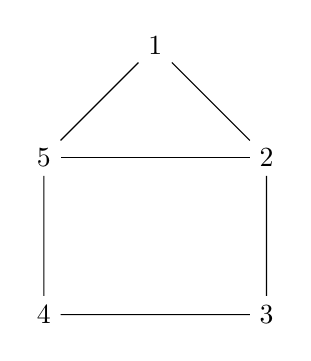
\begin{tikzpicture}[node distance = 2cm]
            \node (1) {$1$};
            \node (2) [below right of=1] {$2$};
            \node (5) [below left of=1] {$5$};
            \node (4) [below of=5] {$4$};
            \node (3) [below of=2] {$3$};
            \draw (1)--(2)--(3)--(4)--(5)--(1);
            \draw (2)--(5);
        \end{tikzpicture}
    \end{figure}
    Then \[
    A_G = \begin{pmatrix} 0&1&0&0&1\\1&0&1&0&1\\  0&1&0&1&0\\0&0&1&0&1\\1&1&0&1&0 \end{pmatrix}.
    \]
\end{example}

\textbf{Fact.} $A_G$ is symmetric and $(A_G)_{x x}=0 ~\forall x \in V(G)$. So $\text{tr}(A)=0$.
\vspace{1mm}

\textbf{Fact.} Let $G$ be a graph and $A_G$ its adjacency matrix. Let $k \in \mathbb{N}$. Then 
\begin{align*}
    (A_G^k)_{xy} = \text{number of walks of length }k \text{ from }x \text{ to }y \text{ in }G.
\end{align*}
\begin{proof}
    If $k=1$, then $xy \in E(G) \iff$ a path of length 1. If $k=2$, then 
    \begin{align*}
        (A_G^2)_{xy} = \sum_{z}^{} (A_G)_{xz} (A)_{zy} = \sum_{z}^{} \mathbbm{1}(x \sim z)\mathbbm{1}(z \sim y) = \text{the number of paths of length 2}.
    \end{align*}
    For $k\ge 3$, proceed by induction.
\end{proof}
We have that $A_G$ acts on $\mathbb{R}^n \to \mathbb{R}^n$ as a linear map. What does this say about $G$?
\begin{example}
    Let $G=C_4$, so $A_G = \begin{pmatrix} 0&1&0&1\\1&0&1&0\\0&1&0&1\\1&0&1&0 \end{pmatrix}$. Take some vector, e.g. $x= \begin{pmatrix} 1&2&-2&3 \end{pmatrix}^\top$. We can think of this as labeling our vertices of the graph.
    Then $A_G x$ is just summing these labels for neighboring vertices, which gives us a new graph with labels $5,-1,5,-1$, i.e. $A_G x = \begin{pmatrix} 5 & -1 & 5 & -1 \end{pmatrix}^\top$.
\end{example}
\textbf{Fact.} If $A$ is a $n \times n$ symmetric matrix, then $A$ has real eigenvalues $\lambda_1 \ge \ldots \ge \lambda_n$. Moreover, there exist eigenvectors $u_1,\ldots,u_n$ which form an orthonormal basis of $\mathbb{R}^n$.
\vspace{1mm}

Thus, given a graph on $n$ vertices, we can talk about its eigenvalues $\lambda_1 \ge \ldots \ge \lambda_n$, which are the eigenvalues of $A_G$. We write $\lambda_{\max} = \lambda_1$ and $\lambda_{\min}= \lambda_n$.
\vspace{1mm}

Note that $\sum_{i=1}^{n} \lambda_i = \text{tr}(A) = 0$, so if $G$ is a nonempty graph, then $\lambda_{\max}>0$ and $\lambda_{\min}<0$.
\vspace{1mm}

Let's compute the eigenvalues of $C_4$. We can check that $\begin{pmatrix} 1&1&1&1 \end{pmatrix}^\top$ is an eigenvector with eigenvalue 2, preferably by thinking about it by summing neighboring labels. We also see that $A_G$ has rank 2, so we have 0 as an eigenvalue and two zero--eigenvectors. Since the eigenvalues sum to zero, the last eigenvalue must be $-2$ (with eigenvector $\begin{pmatrix} 1 & -1 & 1 & -1 \end{pmatrix}^\top$).
\vspace{1mm}

\textbf{Fact.} Let $A$ be a symmetric $n \times n$ matrix. Then 
\begin{align*}
    &\lambda_{\max} = \max_{x \in \mathbb{R}^n\setminus \{0\}} \frac{\langle x, Ax \rangle}{\langle x, x \rangle}\\
    &\lambda_{\min} = \min_{x \in \mathbb{R}^n\setminus \{0\}} \frac{\langle x, Ax \rangle}{\langle x, x \rangle}
\end{align*}
\begin{prop}\label{7.1}
    Let $G$ be a graph.
    \begin{enumerate}[(i)]
        \item If $\lambda$ is an eigenvalue of $G$, then $|\lambda|\le \Delta(G)$.
        \item Let $G$ be connected. Then $\Delta$ is an eigenvalue $\iff G$ is regular, $\mathbbm{1}=\begin{pmatrix} 1,\ldots,1 \end{pmatrix}^\top$ is the corresponding eigenvector, and $\Delta$ has multiplicity 1.
        \item Let $G$ be connected. Then $-\Delta$ is an eigenvalue $\iff G$ is regular and bipartite.
        \item $\lambda_{\max} \ge \delta(G)$.
    \end{enumerate}
\end{prop}
\begin{proof}
    \marginpar{30 Nov 2022, Lecture 24}
    \begin{enumerate}[(i)]
        \item Let $\lambda$ be an eigenvalue with an eigenvector $x=(x_1,\ldots,x_n)^\top$. Let $x_i$ be such that $|x_i|$ is maximal. We may assume that $x_i=1$ by scaling. We have 
        \begin{align*}
            &\lambda = \lambda x_i = (\lambda x)_i = (Ax)_i = (Ax)_i = \sum_{j \sim i}^{} x_j\\
            &|\lambda|= |\sum_{j\sim i }^{} x_j| \le \Delta.
        \end{align*}
        \item ($\impliedby$): If $G$ is regular, then $\mathbbm{1}=(1,\ldots,1)^\top$ is an eigenvector of $G$ with eigenvalue $\Delta$.
        \vspace{1mm}
        
        $(\implies)$: For $\Delta$ is an eigenvalue of $G$, let $x=(x_1,\ldots,x_n)^\top$ be a corresponding eigenvector with $|x_i|$ maximal, and assume $x_i=1$. We have
        \begin{align*}
            \Delta = \Delta x_i = \sum_{j \sim i }^{} x_j \implies \text{deg}(i)=\Delta \text{ and } x_j=1 ~\forall j \sim i.
        \end{align*}
        Now repeat this argument on each of the neighbors of $i$ and continue until we reach every vertex in $G$ (as $G$ is connected) to see that $G$ is $\Delta$--regular and $x=(1,\ldots,1)^\top$. Since we've shown that $\mathbbm{1}$ is the only eigenvector possible for eigenvalue $\Delta$, we conclude that $\Delta$ has multiplicity 1.
        \item $(\impliedby)$: If $G$ is bipartite and regular with bipartition $V(G) = X \sqcup Y$, then $x = (\underbrace{1,\ldots,1}_{|X|}, \underbrace{-1,\ldots,-1}_{|Y|})^\top$ is an eigenvector with eigenvalue $-\Delta$.
        \vspace{1mm}
        
        $(\implies)$: Let $-\Delta$ be an eigenvalue of $G$ with corresponding eigenvector $x=(x_1,\ldots,x_n)$. Let $x_i$ be such that $|x_i|=1$ and assume that $x_i=1$. We have 
        \begin{align*}
            -\Delta = - \Delta x_i = \sum_{j \sim i}^{} x_j \implies \text{deg}(i)=\Delta \text{ and } x_j = -1 ~\forall j \sim i.
        \end{align*}
        Now repeat this for all $j \in N(i)$ to see that $\text{deg}(j)=\Delta$ and all $x_k = 1 ~\forall k \sim j \sim i$. Analogously keep repeating until we reach all vertices in $G$ and see that $G$ is $\Delta$--regular and $x = (1,\ldots,1,-1,\ldots,-1)$ up to a permutation of the coordinates. Moreover, $V(G) = \{j \mid x_j=1\} \cup \{j \mid x_j = -1\}$ defines a bipartition of $G$.
        \item We know that
        \begin{align*}
            \lambda_{\max} = \max_{x \in \mathbb{R}^n\setminus 0}\frac{\langle x,Ax \rangle}{\langle x,x \rangle} \ge \frac{\langle \mathbbm{1},A \mathbbm{1} \rangle}{\langle \mathbbm{1},\mathbbm{1}\rangle} = \frac{1}{n} \sum_{i=1}^{n} \text{deg}(i) \ge \delta(G).
        \end{align*}
    \end{enumerate}
\end{proof}
\begin{defn}
    We say that a graph $G$ is \textbf{$(k,a,b)$--strongly regular} if:
    \begin{itemize}
        \item $G$ is $k$--regular.
        \item For every $xy \in E(G)$, $|N(x) \cap N(y)| = a$.
        \item For every $x \neq y, x \not\sim y$ in $G$, $|N(x) \cap N(y)|=b$.
    \end{itemize}
\end{defn}
\begin{example}
    \begin{itemize}
        \item $C_4$ is $(2,0,2)$--strongly regular.
        \item $C_5$ is $(2,0,1)$--strongly regular.
        \item In fact, any Moore graph is $(k,0,1)$--strongly regular.
    \end{itemize}
\end{example}
\begin{theorem}[Strongly regular graphs are rare]\label{7.2}
    If there exists a $(k,a,b)$--strongly regular graph on $n$ vertices, then 
    \begin{align*}
        \frac{1}{2}\left((n-1) \pm \frac{(n-1)(b-a)-2k}{\sqrt{(a-b)^2+4(k-b)}} \right) \in \mathbb{Z}.
    \end{align*}
\end{theorem}
\begin{proof}
    Let $A$ be the adjacency matrix of a $(k,a,b)$--strongly regular graph on $n$ vertices. Note that 
    \[
    (A^2)_{xy} = \begin{cases}
        a &x \sim y.\\
        b &x \not\sim y, x \neq y.\\
        k &x=y.
    \end{cases}
    \]
    This means that \[
    A^2 = a A + B(J-I-A) + kI,
    \]
    where $J$ is the matrix of all ones. Hence \[
    A^2+(b-a)A+(b-k)I-bJ=0 ~(\dagger).
    \]
    We know by Proposition \ref{7.1} that $k$ is an eigenvalue of $A$ with corresponding eigenvector $\mathbbm{1}=(1,\ldots,1)^\top$ and $k$ has multiplicity $1$. Let $\lambda$ be an eigenvalue with $\lambda \neq k$, and let $x$ be a corresponding eigenvector. Multiply $(\dagger)$ by $x$ to get that \[
    \lambda^2 x + \lambda(b-a)x + (b-k)x = 0
    \]
    since $Jx = 0$, since $x \perp \mathbbm{1}$. Hence
    \begin{align*}
        &\lambda^2+\lambda(b-a)+(b-k)=0 \\
        &\implies \lambda = \frac{1}{2} \left((a-b) \pm \sqrt{(b-a)^2 + 4(k-b)}\right).
    \end{align*}
    Let $\lambda,\mu$ be the solutions to this quadratic equation and assume that $\lambda$ has multipllicity $s$ and $\mu$ has multiplicity $t$. % *writes mu*. "FUCK, t"
    We have 
    \begin{align*}
        k + s \lambda + t \mu = \sum_{i=1}^{n} \text{tr}(A) = 0,
    \end{align*}
    hence
    \begin{align*}
        \begin{cases}
            &s \lambda + t \mu = -k\\
            &s + t = n-1.
        \end{cases} 
    \end{align*}
    Solve these for $s,t \in \mathbb{Z}$ to get the number in our theorem as desired.
\end{proof}
\begin{cor}
    Let $G$ be a Moore graph with $\Delta(G)=k$. Then $k \in \{2,3,7,57\}$.
\end{cor}
\begin{proof}
    The idea is that if $G$ is a Moore graph, then it is $(k,0,1)$--strongly regular on $k^2+1$ vertices. Hence we have \[
    \frac{1}{2}\left(k^2 \pm  \frac{k^2-2k}{\sqrt{4k-3}}\right) \in \mathbb{Z},
    \]
    which gives $k \in \{2,3,7,57\}$.
\end{proof}

\end{document}